%%%%%%%%%%%%%%%%%%%%%%%%%%%%%%%%%%%%%%%%%%%%%%%%%%%%%%%%%%%%%%%%%%%%%%%%%%%%
% AGUtmpl.tex: this template file is for articles formatted with LaTeX2e,
% Modified September 2012
%
% This template includes commands and instructions
% given in the order necessary to produce a final output that will
% satisfy AGU requirements.
%
% PLEASE DO NOT USE YOUR OWN MACROS
% DO NOT USE \newcommand, \renewcommand, or \def.
%
% FOR FIGURES, DO NOT USE \psfrag or \subfigure.
%
%%%%%%%%%%%%%%%%%%%%%%%%%%%%%%%%%%%%%%%%%%%%%%%%%%%%%%%%%%%%%%%%%%%%%%%%%%%%
%
% All questions should be e-mailed to latex@agu.org.
%
%%%%%%%%%%%%%%%%%%%%%%%%%%%%%%%%%%%%%%%%%%%%%%%%%%%%%%%%%%%%%%%%%%%%%%%%%%%%
%
% Step 1: Set the \documentclass
%
% There are two options for article format: two column (default)
% and draft.
%
% PLEASE USE THE DRAFT OPTION TO SUBMIT YOUR PAPERS.
% The draft option produces double spaced output.
%
% Choose the journal abbreviation for the journal you are
% submitting to:

% jgrga JOURNAL OF GEOPHYSICAL RESEARCH
% gbc   GLOBAL BIOCHEMICAL CYCLES
% grl   GEOPHYSICAL RESEARCH LETTERS
% pal   PALEOCEANOGRAPHY
% ras   RADIO SCIENCE
% rog   REVIEWS OF GEOPHYSICS (if you encounter problems with this class file, use jgrga instead)
% tec   TECTONICS
% wrr   WATER RESOURCES RESEARCH
% gc    GEOCHEMISTRY, GEOPHYSICS, GEOSYSTEMS
% sw    SPACE WEATHER
%
% For JOURNAL OF ADVANCES IN MODELING EARTH SYSTEMS, use jgrga.
%
%
% (If you are submitting to a journal other than jgrga,
% substitute the initials of the journal for "jgrga" below.)

\documentclass[draft,jgrga]{agutex}

%%%%%%%%%%%%%%%%%%%%%%%%%%%%%%%%%%%%%%%%%%%%%%%%%%%%%%%%%%%%%%%%%%%%%%%%%
% OPTIONAL:
% To produce a two-columned version:
%\documentclass[jgrga]{AGUTeX}

% Two-columned format can be used to estimate the number of pages
% for the final published PDF.

% PLEASE USE THE DRAFT OPTION TO SUBMIT YOUR PAPERS.
%%%%%%%%%%%%%%%%%%%%%%%%%%%%%%%%%%%%%%%%%%%%%%%%%%%%%%%%%%%%%%%%%%%%%%%%%
% OPTIONAL:
% To create numbered lines:

% If you don't already have lineno.sty, you can download it from
% http://www.ctan.org/tex-archive/macros/latex/contrib/ednotes/
% (or search the internet for lineno.sty ctan), available at TeX Archive Network (CTAN).
% Take care that you always use the latest version.

% To activate the commands, uncomment \usepackage{lineno}
% and \linenumbers*[1]command, below:

\usepackage{lineno}
\usepackage{gensymb}
\linenumbers*[1]

%  To add line numbers to lines with equations:
% \begin{linenomath*}
%\begin{equation}
%\end{equation}
%\end{linenomath*}
%%%%%%%%%%%%%%%%%%%%%%%%%%%%%%%%%%%%%%%%%%%%%%%%%%%%%%%%%%%%%%%%%%%%%%%%%
% Figures and Tables
%
% When submitting articles through the GEMS system:
% COMMENT OUT ANY COMMANDS THAT INCLUDE GRAPHICS.
% (See FIGURES section near the end of the file.)
%
% DO NOT USE \psfrag or \subfigure commands.
%
%  Figures and tables should be placed AT THE END OF THE ARTICLE,
%  after the references.
%
%  Uncomment the following command to include .eps files
%  (comment out this line for draft format):
\usepackage{graphicx}
%
%  Uncomment the following command to allow illustrations to print
%   when using Draft:
%\setkeys{Gin}{draft=True}
%
% Substitute one of the following for [dvips] above
% if you are using a different driver program and want to
% proof your illustrations on your machine:
%
% [xdvi], [dvipdf], [dvipsone], [dviwindo], [emtex], [dviwin],
% [pctexps],  [pctexwin],  [pctexhp],  [pctex32], [truetex], [tcidvi],
% [oztex], [textures]
%
% See how to enter figures and tables at the end of the article, after
% references.
%
%%%%%%%%%% Start TeXmacs macros
\usepackage{amsmath,bbm}
\newcommand{\nonesep}{}
\newcommand{\tmem}[1]{{\em #1\/}}
\newcommand{\tmop}[1]{\ensuremath{\operatorname{#1}}}
\newcommand{\tmsamp}[1]{\textsf{#1}}
\newcommand{\tmstrong}[1]{\textbf{#1}}
\newcommand{\tmtextit}[1]{{\itshape{#1}}}
\newcommand{\parby}[2]{\ensuremath{\frac{\partial #1}{\partial #2}}}
\newcommand{\E}{\ensuremath{\vec{E}}}
\newcommand{\V}{\ensuremath{\vec{v}}}
\newcommand{\U}{\ensuremath{\vec{u}}}
\newcommand{\B}{\ensuremath{\vec{B}}}
\newcommand{\J}{\ensuremath{\vec{J}}}
\newcommand{\Vper}{\ensuremath{\vec{v}_{\perp}}}
\newcommand{\Vpara}{\ensuremath{\vec{v}_{\parallel}}}
\newcommand{\Uper}{\ensuremath{\vec{u}_{\perp}}}
\newcommand{\Upara}{\ensuremath{\vec{u}_{\parallel}}}
\newcommand{\X}{\ensuremath{\vec{x}}}
\newcommand{\DIV}{\ensuremath{\nabla \cdot}}
\newcommand{\CURL}{\ensuremath{\nabla \times}}
%%%%%%%%%% End TeXmacs macros
\usepackage{setspace}
%% ------------------------------------------------------------------------ %%
%
%  ENTER PREAMBLE
%
%% ------------------------------------------------------------------------ %%

% Author names in capital letters:
\authorrunninghead{WILTBERGER ET AL.}


% Shorter version of title entered in capital letters:
\titlerunninghead{Effects of ET}

%Corresponding author mailing address and e-mail address:
%\authoraddr{Corresponding author: A. B. Smith,
%Department of Hydrology and Water Resources, University of
%Arizona, Harshbarger Building 11, Tucson, AZ 85721, USA.
%(a.b.smith@hwr.arizona.edu)}
\authoraddr{Corresponding author: M. Wiltberger,
National Center for Atmospheric Research,
High Altitude Observatory,
3080 Center Green,
Boulder, CO 80301
(wiltbemj@ucar.edu)}
\paperid{???}
\begin{document}

\def\oplus{O$^+$ }
\def\hplus{H$^+$ }
\def\heplus{He$^+$}
\def\nplus{N$^+$}
\def\dst{$D_{ST}$ }


%% ------------------------------------------------------------------------ %%
%
%  TITLE
%
%% ------------------------------------------------------------------------ %%


\title{Effects of Electrojet Turblence in simulations of the March 17, 2013 Geomagnetic Storm}
%
% e.g., \title{Terrestrial ring current:
% Origin, formation, and decay $\alpha\beta\Gamma\Delta$}
%

%% ------------------------------------------------------------------------ %%
%
%  AUTHORS AND AFFILIATIONS
%
%% ------------------------------------------------------------------------ %%


%Use \author{\altaffilmark{}} and \altaffiltext{}


% \altaffilmark will produce footnote;
% matching \altaffiltext will appear at bottom of page.

% \authors{A. B. Smith,\altaffilmark{1}
% Eric Brown,\altaffilmark{1,2} Rick Williams,\altaffilmark{3}
% John B. McDougall\altaffilmark{4}, and S. Visconti\altaffilmark{5}}

%\altaffiltext{1}{Department of Hydrology and Water Resources,
%University of Arizona, Tucson, Arizona, USA.}

%\altaffiltext{2}{Department of Geography, Ohio State University,
%Columbus, Ohio, USA.}

%\altaffiltext{3}{Department of Space Sciences, University of
%Michigan, Ann Arbor, Michigan, USA.}

%\altaffiltext{4}{Division of Hydrologic Sciences, Desert Research
%Institute, Reno, Nevada, USA.}

%\altaffiltext{5}{Dipartimento di Idraulica, Trasporti ed
%Infrastrutture Civili, Politecnico di Torino, Turin, Italy.}

\authors{M. Wiltberger, \altaffilmark{1}
V. Merkin, \altaffilmark{2}
B. Zhang,   \altaffilmark{1}
F. Toffletto,  \altaffilmark{3}
M. Oppenheim,  \altaffilmark{4}
W. Wang,  \altaffilmark{1}
J. G. Lyon, \altaffilmark{5}
J. Liu,  \altaffilmark{1}
and Y Dimant \altaffilmark{4}
}

\altaffiltext{1}
{High Altitude Observatory, National Center for Atmospheric Research,Boulder, Colorado, USA.}

\altaffiltext{2}{Applied Physics Laboratory, Johns Hopkins University, MD, USA.}

\altaffiltext{3}{Department of Physics and Astronomy, Rice University, TX, USA.}

\altaffiltext{4}{2Center for Space Physics, Boston University, Boston, Massachusetts, USA}

\altaffiltext{5}{Department of Physics and Astronomy, Dartmouth College,Hanover, NH, USA.}
%

%% ------------------------------------------------------------------------ %%
%
%  ABSTRACT
%
%% ------------------------------------------------------------------------ %%

% >> Do NOT include any \begin...\end commands within
% >> the body of the abstract.

\begin{abstract}
Examines the impacts of including Electrojet Turbulence (ET) in simulations of to the geomagnetic storm that occurred on 17 March 2013.   We see many cool things.

\end{abstract}

%% ------------------------------------------------------------------------ %%
%
%  BEGIN ARTICLE
%
%% ------------------------------------------------------------------------ %%

% The body of the article must start with a \begin{article} command
%
% \end{article} must follow the references section, before the figures
%  and tables.

\begin{article}

%% ------------------------------------------------------------------------ %%
%
%  TEXT
%
%% ------------------------------------------------------------------------ %%

\section{Introduction}

Initial drafting of this section has been assigned to Meers and Slava.

\section{Simulation Setup}
\label{sec-model-sims}
This study focuses on using the geomagnetic storm that occurred on 17 March 2013 as a case study for two new features of the LFM-RCM geospace model.   As previously discussed the LFM-RCM model combines the Lyon-Fedder-Mobarry MHD model of the magnetosphere with the Rice Convection Model of the inner magnetosphere and the Mangetosphere-Ionosphere Coupler Solver of ionospheric electrodynamics to provide a tightly coupled model of the geospace system. \cite{Pembroke:2012gc} describes in detail the basic process of coupling these three models together during idealized solar wind conditions with modest solar wind driving and no dipole tilt.  Section \ref{sec-lfm-rcm} describes how this approach has been modified to include realistic solar wind conditions, including nonzero IMF $B_Y$, as well as variations in the Earth's dipole tilt.  \cite{2005GeoRL..3222101M} implemented an adjustment to the ionospheric conductances based upon the theoretical analysis of the Farley-Buneman instability (FBI) conducted by \cite{2003JGRA..108.1350D}.  This capability has not been widely used in LFM simulations, but is being made part of the LFM-RCM geospace model.  Section \ref{sec-ET} discusses how both the Anomalous Electron Heating (AEH) and Non-Linear Current (NLC) aspects of the Electrojet Turbulence are implemented in the MIX portion of the LFM-RCM model.  Next we present the results of simulations for a geomagnetic storm that occurred on 17 March 2013.  We compare and contrast the results of LFM-RCM simulations with and without the Electrojet Turbulence including comparisons with a range of observations.  The final section of the paper we discuss our results and next steps.

\subsection{LFM-RCM}
\label{sec-lfm-rcm}

\cite{Pembroke:2012gc} provides a detailed description of the coupling process between the LFM, MIX and RCM models for simulations of geospace.  Since that study used idealized solar wind conditions with no dipole tilt after reviewing the basics of the LFM-RCM coupling this section will address the changes made to coupling infrastructure needed to allow model to work for realistic solar wind conditions and dipole tilts.  

The fundamental aspect of the model coupling is an exchange of magnetic field and plasma information in the inner magnetosphere to RCM from LFM and then an update of the plasma information from RCM to the LFM.  The MIX model is providing ionospheric potential information to both the LFM and RCM models.  All of the exchanges use the Center for Integrated Space Weather Modeling (CISM)  coupling infrastructure  and that infrastructure is utilized in the update version \citep{2004JASTP..66.1469G}.  To transfer information from the LFM to the RCM the LFM computes time averages of the pressure, density and magnetic field over an exchange interval. The averaged fields are interpolated onto an intermediate regular Cartesian grid.  This intermediate grid is then used to calculated field line-averaged pressure and density for positions in the RCM's ionospheric grid.  A key innovation of the \cite{Pembroke:2012gc} was the implementation of the plasma-$\beta$ methodology for setting the location of the outer boundary of the RCM.  This switch, which essentially prevented the RCM from computing regions with large flows, remains active in the storm simulations we present in this paper.   After the RCM computes its plasma pressures and densities these values are transferred back to the LFM once again using the intermediate grid.  The RCM density model includes a modifications to a fit of static plasmasphere model of \cite{Gallagher:2000p2797}.  At this time we have not implemented a dynamic plasmasphere calculation, but that is logical next step for improvement of the coupled model.  Another set of field line traces from the RCM ionospheric grid points are used to determine the local values on intermediate grid and than those values are interpolated to LFM grid points.  The mapping back to LFM assumes that the distribution of plasma density and pressure  is constant along field lines. As before the RCM values do not immediately replace the LFM values, instead they bled into the LFM over the exchange time interval.  It is important to note that the previous work used a 1-minute exchange interval as a  balance between speed and accuracy.  For strong solar wind driving conditions we have found it necessary to reduce the coupling interval to 15-seconds. 

The first major modification to the previous coupling efforts is in support of including dipole tilts in the calculation of the coupled model.  The LFM-MIX model has long had support for conducting simulations with realistic dipole tilts.  This is done by continuing to have the dipole axis of the Earth aligned with the Z-axis of the computational model and inputing the solar wind conditions in SM coordinates.  As \cite{1992P&SS...40..711H} explains the SM coordinate system has the Z-axis parallel to the north magnetic pole and transformation between this coordinate system and the more commonly used GSM coordinate system is simply rotation about the Y-axis by the dipole tilt angle.   The cartesian intermediate grid is setup in SM coordinates for the transfer of data to and from the LFM to RCM the ionospheric foot points are transformed from geographic coordinates to SM coordinates using the GEOPACK coordinate transform package.    The RCM typically includes the effects of the corotation potential which is not part of stand alone LFM-MIX, but is enabled when coupled with the RCM. 

The second key modification of the LFM-RCM coupling is how the asymmetries in the ionosphere are addressed.  In the MIX module the ionospheric potential for the northern and southern hemispheres are calculated independently.  The field-aligned current patterns taken from the global MHD simulation are shared between the hemispheres, but the ionospheric conductances can be different.  The first major difference comes from the implementation of a EUV conductance model that calculates the local value of the Hall and Pedersen conductance based upon the solar zenith angle and the F107 flux value.  We have adapted the approach used by Assimilative Mapping of Ionospheric Electrodynamics  (AMIE) for the MIX module \citep{1992AdSpR..12...59R}.  The ionospheric conductance model also includes an empirical model for electron precipitation.  As described by \cite{2009JGRA..11401204W} this model includes modifications of the precipitation values based upon the local EUV conductance values allowing the model to simulate seasonal variations of particle precipitation and their impacts on geospace system.  On the other hand the RCM assumes that there are no differences between the northern and southern hemispheres.  

The compromise solution we have adopted for the version of the coupled simulations present here works as follows.  The low latitude boundary of the the ionospheric solution for electrodynamic solver is extended equatorward from 45\degree ~to 60\degree ~colatitude.   The 45\degree ~boundary corresponds to dipole mapping of the 2 $R_E$ inner boundary of the MHD solution grid within the LFM.  The 60\degree ~boundary corresponds to the low latitude boundary for the RCM ionospheric calculation. {\em Frank - Is the previous statement correct?} For the northern hemisphere the typical low latitude boundary condition of assuming that potential is zero is used.  The northern hemispheric values for the potential as well as the average energy and flux of precipitating electrons are then stored for latter passage to the RCM for its calculation.  The computation of the southern hemisphere potential is done down 45\degree ~with the low latitude boundary value being set of the potential obtained from the northern hemisphere at that location.   By setting the southern hemisphere boundary with the northern hemisphere values we are attempting ensure that closed field lines in the calculation have the same potential values.   {\em Slava and Frank - Is that the best way to describe the motivation for this coupling approach?  Also, should we address why we aren't passing any kind of aggregate flux or conductance information to the RCM calculation.}

As a quick side note we take a moment to compare our approach that utilized by other groups to couple global MHD models with the RCM.  The Space Weather Modeling Framework \cite{2005JGRA..11012226T} to couple the MHD magnetosphere solution to inner magnetosphere models.   \cite{2004JGRA..10912219D} did the initial work coupling the RCM with the BATS-R-US magnetosphere solution.  Like us they used field line tracing to compute flux tube quantities for transfer between the two components and also assume the plasma parameters are constant along field lines.  They support exchange intervals between 10 seconds to 10 minutes with the choice of exchange intervals between models being driving by the strength of  convection within the event being simulated.  This initial work was done for simulations with no dipole tilts and uniform ionospheric conductances.   \cite{2010SpWea...803002W} presents validation studies comparing the magnetic field and plasma parameters for a set of geomagnetic storms.  While these results clearly include the effects of dipole tilts and particle precipitation effects the study does not provide any details on how these conditions are handled in the coupled model.   More recently \cite{Glocer:2013dv} documented the two-way coupling of the Comprehensive Ring Current Model (CRCM) with the BATS-R-US global magnetosphere model, while they presented results for 22 July 2009 geomagnetic storm the paper does not discuss the details of how dipole tilt is addressed.  {\em Frank and Slava - I thought this was a worth while addition here and not in the introduction since it concentrates on coupling details.  Am I being to harsh in my language about not discussing how the dipole tilt is addressed? I'm not aware of any OpenGGCM publications with RCM.  If I've missed something please let me know.}

\subsection{Electrojet Turbulence Implementation}
\label{sec-ET}

\cite{2011JGRA..116.9304D} developed a model of how FBI turbulence modifies E-region conductivities when driven by strong DC electric fields.  This turbulence gives rise to both nonlinear currents (NC) and anomalous electron heating (AEH). Both these will increase the conductivity. This model was incorporated into the MIX module as a set
of conductance correction factors that depend on the driving electric field.

The model of AEH was developed in \cite{2003JGRA..108.1350D} assuming a specific FBI turbulence level. This self-consistent approach accounts for the fact that as the FBI turbulence raises the electron temperature $T_e$, it increases the instability threshold field, $E_{\mathrm{Thr}}^{\min}$, causing the saturated turbulence level to grow with $E_0$ much more slowly than if $T_e$ were constant. It also accounted for kinetic modification of the electron distribution function and the corresponding enhanced cooling this causes.  The resulting elevated electron temperature $T_{e}$ increases the conductivities by reducing in the local plasma recombination rate and therefore increasing the plasma density \cite{1978SVPCS..10.....G,1990AdSpR..10..239S,2003JGRA..108.1350D,2006GeoRL..3313809M}.

The NC model was developed by \cite{1996GeoRL..23.3333O,1997AnGeo..15..899O}.  This predicts a strong current driven by FB turbulence in the direction of the DC field.  The model used in the MIX module combines $E_{\mathrm{Thr}}^{\min}(E)$ with an assumed level of saturated FBI density fluctuations as seen in simulations by \cite{2013JGRA..118.1306O}. This modifies the Hall and Pedersen conductance, as described in \cite{2011JGRA..116.9304D}.

Inside the MIX module we have implemented the following conductivity correction terms combing the AEH and NC correction factors.   In regions where the electric field is greater than 35 mV/m we have implemented, 

\begin{equation}
\label{eq-sigmap-fbi}
\Sigma_P^{ET} = \Sigma_P^O(1+0.01 (E - 35) + 1.3e10^{-5}(E - 35)^2),
\end{equation}

as the calculation for the Electojet Turbulence (ET) modified conductivity, $\Sigma_P^{ET}$.  In Equation \ref{eq-sigmap-fbi} $E$ is the ionospheric electric field in mV/m and $\Sigma_P^O$ is the Pedersen conductivity obtained from the baseline ionospheric model and includes both the EUV and electron precipitation terms.  This multiplier includes the effect of the temperature driven recombination reduction as well as the that of nonlinear current.  The FBI modified Hall conductivity, $\Sigma_H^{ET}$ ,  is simply 

\begin{equation}
\label{eq-sigmah-fbi}
\Sigma_H^{ET} = \Sigma_H^O(1+0.01172 (E - 35) - 1.207e10^{-5}(E - 35)^2),
\end{equation}

where $\Sigma_H^O$ is the baseline Hall conductivity.   Figure \ref{fbi-multi-fig} shows the effects of these multipliers over a range electric fields.  The Pedersen multiplier (blue curve) is nearly linear over the range from 35-200 mV/m reaching a peak value of 3.0 at 200 mV/m.  The Hall multiplier has a negative coefficient on the the squared term and so falls of more dramatically at higher values of the electric field.  It reaches a value of 2.3 at 200 mV/m.  We note that the Farley-Buneman Instability typically starts developing if the convection field, $E$, exceeds $\approx20$ mV/m. However, the macroscopic effect of E-region turbulence becomes substantial only for field when it exceeds $E>35$ mV/m, therefore we eliminate the effect below this level for computational simplicity. 

\begin{figure}
\noindent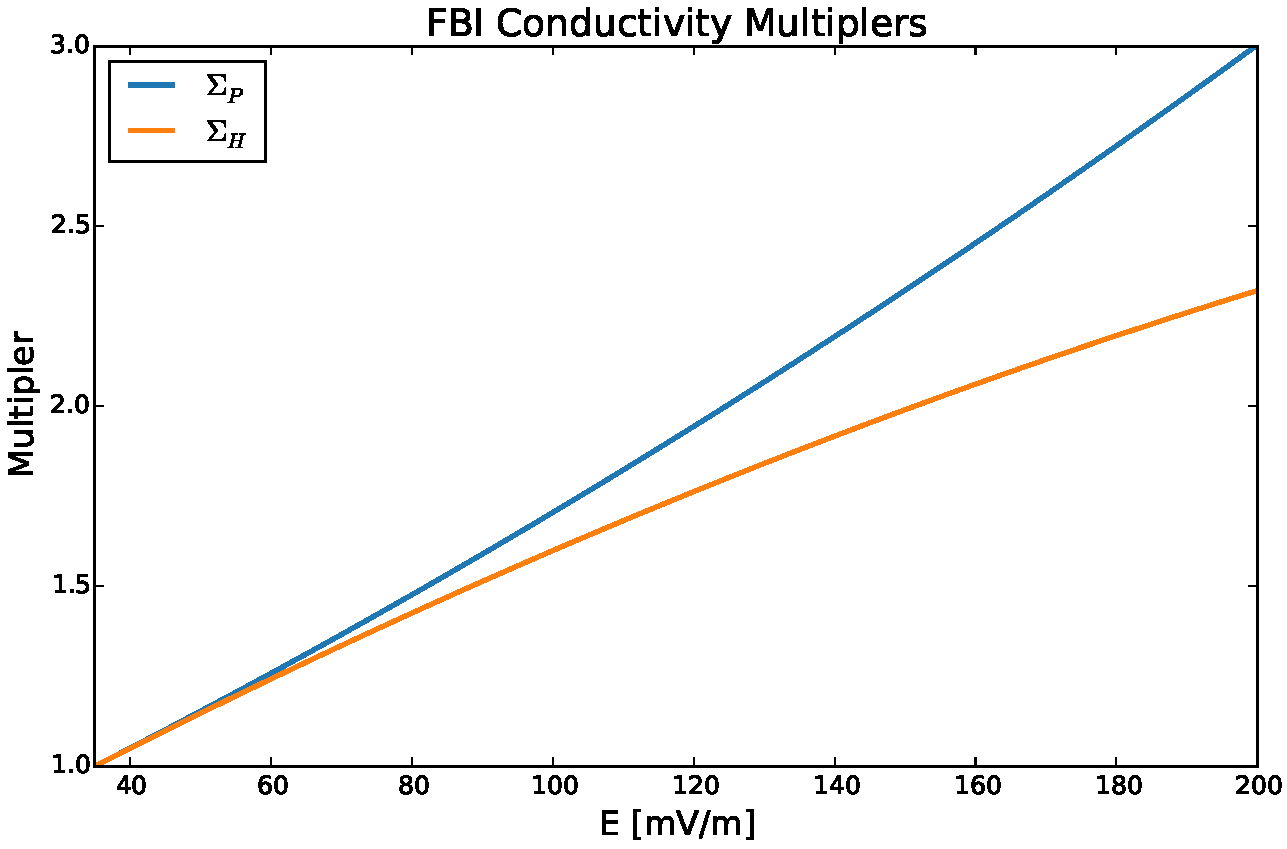
\includegraphics[width=20pc]{JGRPaper-ConductMulti.pdf}
\caption{\label{fbi-multi-fig} 
The conductivity multipliers for the Electrojet Turbulence effects.  The blue curve is for the Pedersen conductivity while the orange curve is for the Hall conductivity.  The effects occur for all values above 35 mV/m.  } 
\end{figure}

\subsection{17 March 2013 Simulation}
\label{sec-17mar13}

On 17 March 2013 an interplanetary coronal mass ejection arrived at the Earth and drove a significant geomagnetic storm, $D_{ST} < -100$, over the next day.  Solar wind conditions obtained from the OMNI dataset were used to drive the LFM-RCM model and those are shown in Figure \ref{sw-fig}.  Prior to the shock preceding the CME the solar wind conditions are fairly typical, namely density $\approx$5 cc, velocity $\approx$425 km/s, with interplanetary magnetic field (IMF) weak, $<$ 5nT in magnitude, mainly in the northward direction.  At 05:55 UT a shock is clearly present in the solar wind with $V_X$ GSM reaching -650 km/s and the density increasing to 10 cc.  In the next three hours the IMF is variable, with IMF $B_Z$ mainly southward reaching values of -20 nT, but having significant intervals with northward IMF.  The Y component of the IMF has similar magnitude in amplitude and appears to have a 180 $\deg$ phase shift.  After approximately  09:00 UT on the 17th the Y and Z components become more in phase and slowly reduce in amplitude reaching typical values by the end of the day.  After about 12:00 UT the solar wind speed slowly begins to decrease reaching a value of about 550 km/s by the end of 17 March.

The LFM-RCM simulations for this interval where run using solar wind conditions from Figure \ref{sw-fig}.  As previously discussed the LFM uses a non-orthogonal spherical mesh for the grid.  The simulations conducted here use 106 radial, 96 azmiuthal, and 128 polar cells.  This quad resolution version of the LFM contains twice as many cells as the results reported by \cite{Pembroke:2012gc} initial work with coupling LFM-RCM.   The RCM simulations where done on a grid with XX and YY points.  The intermediate transfer grid between LFM-RCM used for the field line tracing had a resolution of ZZ.  In the MIX ionospheric solution the ionospheric resolution was increased from a 2x2$^{\circ}$ resolution to 1x1$^{\circ}$resolution.  The full ionospheric conductance model described by \cite{2009JGRA..11401204W} by was enabled in the MIX calculations.  We ran two sets of simulations.  The first hereafter, baseline, used the standard ionospheric model.  The second, hereafter ET, had the Electrojet Turbulence implementation discussed in Section \ref{sec-ET} enabled.  The solar wind driving, grid resolution, and all other model parameters are not changed between these two runs. 

\begin{figure}
\noindent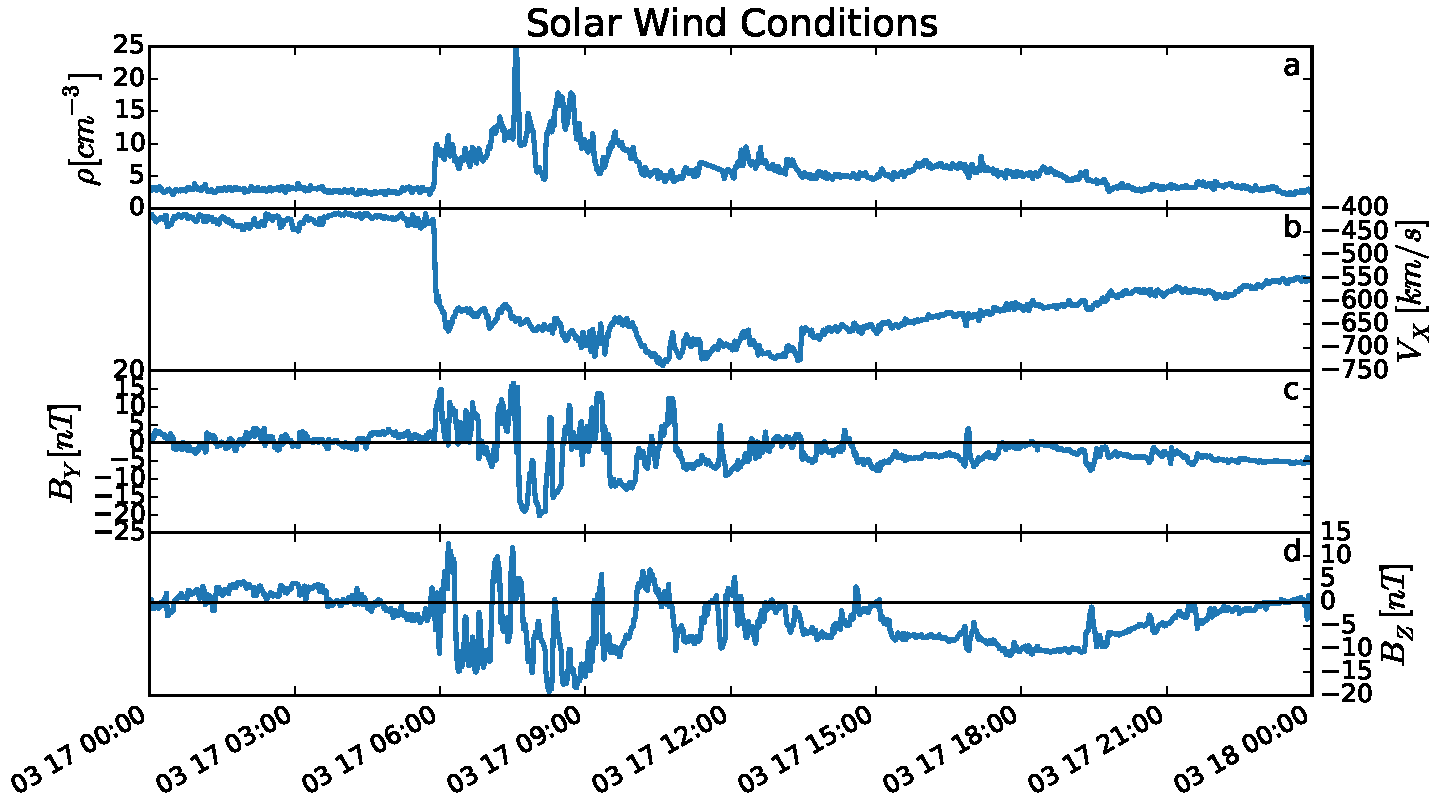
\includegraphics[width=20pc]{JGRPaper-SWFig.pdf}
\caption{\label{sw-fig} 
Solar wind and IMF conditions during the 17 March 2013 geomagnetic storm event.  Panel a) shows the number density, b) the $V_X$ in GSM coordinates.  The IMF GSM Y and Z values are plotted in panels c) and d) respectively.} 
\end{figure}

\section{Analysis of results}
\label{sec-analysis}
We now move on to present the results of from the two simulations for the St Patrick's Day 2013 storm event.  We begin, in Section \ref{sec-comp}, with a broad overview of the results of the simulation including comparisons of ionospheric structures and global measures.  After this overview of the event and simulation results we move onto make comparisons between the simulation results and observations.  In Section \ref{sec-dmsp} we make detailed comparisons between the simulation results and Defense Meteorological Satellite Program (DMSP) observations during the peak of the storm.  These results show ability of the model capture features associated with Sub-Auroral Polarization Streams (SAPS).  Next, we assess the ability of the model to simulate field aligned currents (FACs) by compare the results with patterns obtained from the AMPERE mission.  Finally, in Section \ref{sec-ts07d} we examine the structure of the inner magnetospheric pressures associated with the ring current by comparing the results with those obtain from the TS07-D empirical magnetic field model.

\subsection{Baseline versus ET}
\label{sec-comp}

Figure \ref{ion-pattern-fig} is frame extracted from the scientific visualization that is included in auxiliary materials that are part of the online version of this article.  The top row figure shows the results from the baseline simulation while the bottom row shows the results from ET simulations.  Panels a) and d) of Figure \ref{ion-pattern-fig} provide a comparison between the cross polar cap potential patterns and the structure of the field aligned currents for the northern hemisphere during the course of the magnetic storm.   In the snapshot taken at 10:00 UT on March 17th the region-1 and region-2 FAC current structures are clearly apparent.  The cross polar cap potential is weaker in the ET run, but the alignment of the pattern in confinement to high-latitudes by the region-2 currents is consistent in both simulation results.  The second column, panels b) and e), shows the Pedersen conductance.  In both runs the EUV ionization  profile is apparent on the dayside along with auroral oval structure driven by the empirical precipitation model.  It's also clear at this snapshot that the ET model is having an impact because the Pedersen conductance in the auroral oval is larger in the ET results.  The final column of Figure \ref{ion-pattern-fig}, panels c) and f), provides a comparison between the Hall conductances.  Just like in Pedersen conductance the EUV profile and auroral oval are apparent.  It is important to note that when comparing the conductance plots that color ranges are the same across simulations for each type of conductance, but the Hall conductance upper limit is a factor of two larger than the Pedersen conductance in order to make the differences between the different simulations more apparent.

\begin{figure*}[t]
\noindent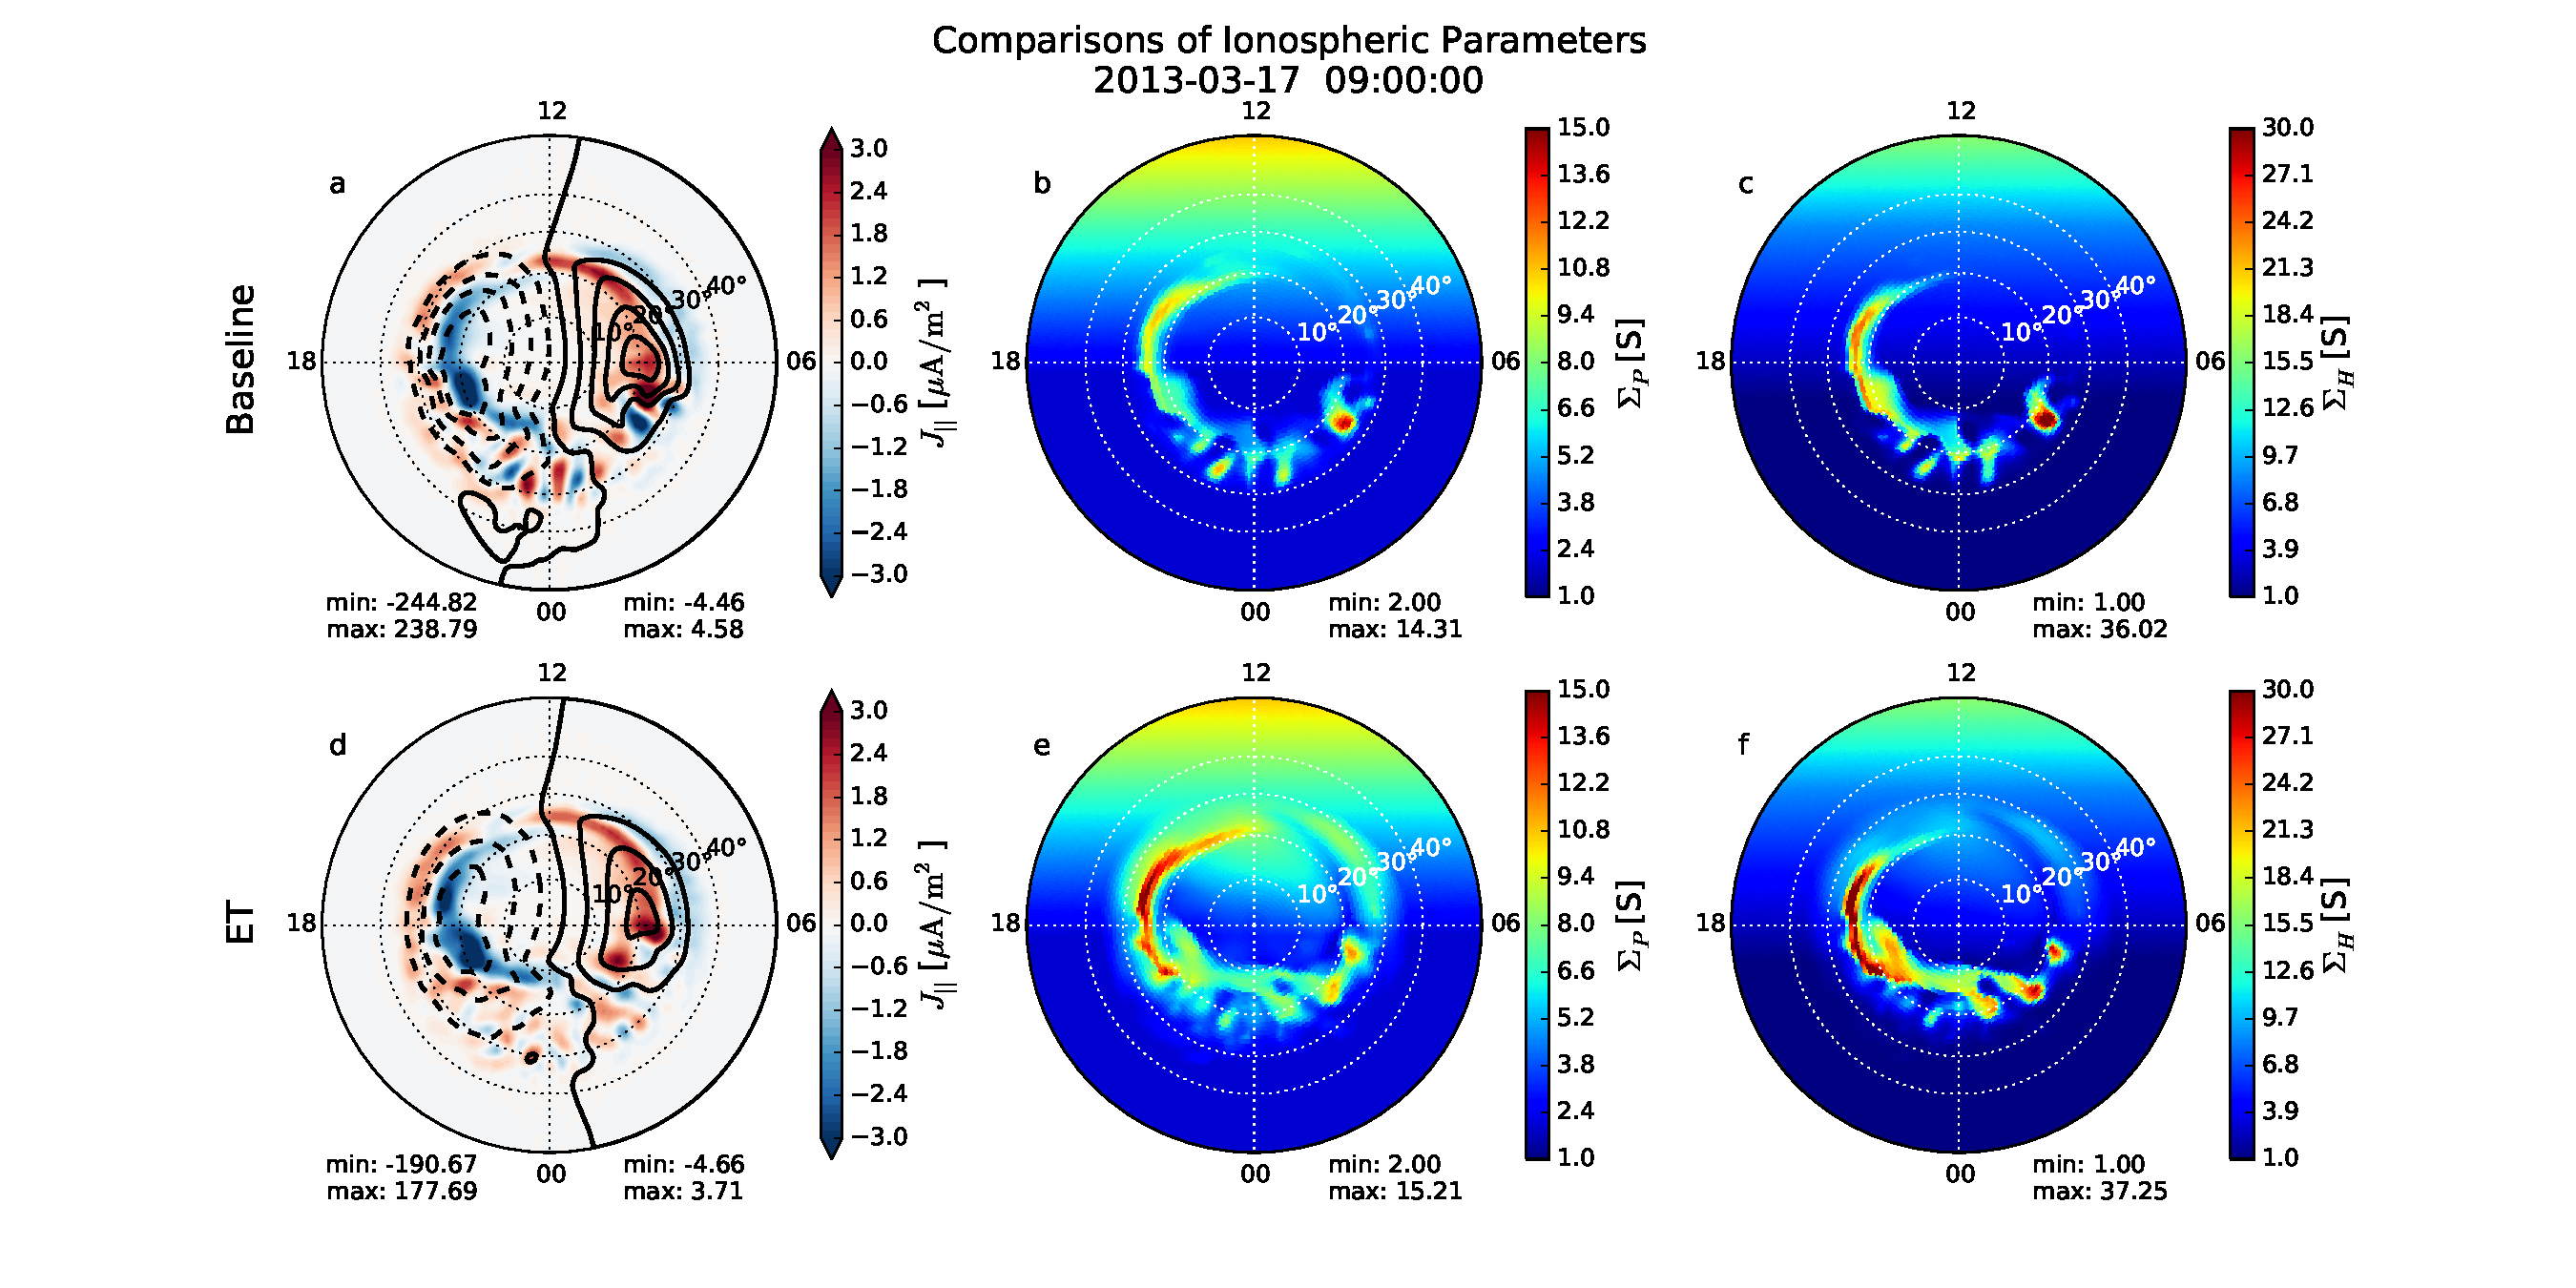
\includegraphics[width=39pc]{JGRPaper-IonPatterns.pdf}
\caption{\label{ion-pattern-fig}
Frame from the scientific visualization showing of FAC and CPCP as well as Pedersen and Hall conductivities for the Baseline and ET simulations of the 17 March 2016 geomagnetic storm.  The top row (panels a-c) contains the results from the baseline simulation while the bottom row (panels d-f) contains the results of the simulation with the ET enabled.  The first column (panels a and d) has the FAC in color with blue being upward and red being downward as well as the CPCP pattern with 20 kV contours.  The middle column (panels b and e) contains the Pedersen conductivity.  The last column (panels c and f) contains the Hall conductivity.  The color bar for the Pedersen conductance ranges from 1 to 15 [S] while the upper limit for the Hall conductance is 30 [S]}
\end{figure*}

Before moving on to examine the evolution of the ionospheric parameters in the simulation during the course of the magnetic storm we turn our attention to Figure \ref{ion-comp-fig} that shows a comparison of several global diagnostic parameters over the course of the storm.  The top panel, a), shows the time history of the cross polar cap potential obtained by taking the difference of the max and min of the potential at each dump step.  Using a convention that will be maintained throughout this paper the baseline simulation results are sown with the green line and the ET simulation results are shown with the purple line.  The second panel, b), of the Figure shows the strength field-aligned current obtained by integrating the positive FAC over the northern hemisphere at each time step.  Panel c) at the bottom of Figure \ref{ion-comp-fig} shows a comparison between the simulation results and observations for the $D_{ST}$ index.  The simulated $D_{ST}$ index was calculated using Biot-Savart method that determines the ground magnetic field perturbations driven by the magnetospheric, field-aligned, and ionospheric currents.  Also shown in this panel is observed $D_{ST}$ index obtained from CDAweb database.   Following the convention for this paper the observed $D_{ST}$ index is shown with a blue line.

\begin{figure}
\noindent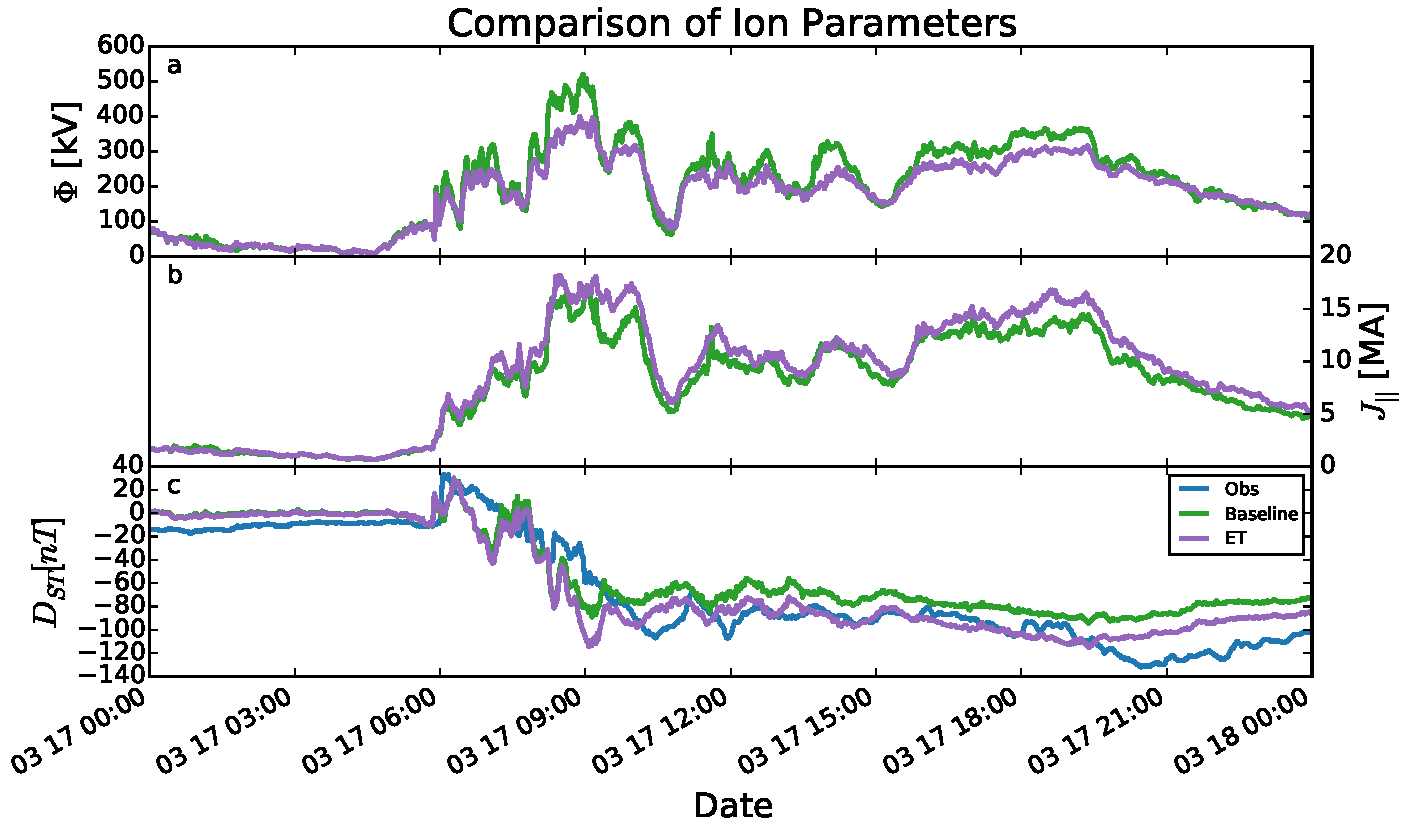
\includegraphics[width=20pc]{JGRPaper-IonFig.pdf}
\caption{\label{ion-comp-fig} 
Comparison of the CPCP, FAC, and $D_{ST}$ time series for the storm event for the Northern hemisphere.  Panel a at the top shows the CPCP in kV.  The middle panel (b) has the integrated  FAC.  Panel c at the bottom has the $D_{ST}$ index.  In each panel the LFM-RCM results are shown with the green line, the ET results with the purple line.  In the bottom panel the $D_{ST}$ obtained from CDAWeb is plotted in blue} 
\end{figure}

The solar wind conditions prior to the 05:50 UT arrival of the shock preceding the CME are modest with velocity around 420 [km/s], density slight above 3 [cc] and the IMF mainly northward with a small $B_Y$ component.  The scientific visualization of the ionospheric parameters begins at 00:00 UT on March 17th and results shown between then and the arrival of the shock show little difference between the two simulations.   For example at 03:00 UT both simulations show a NBZ current system in the ionosphere with very weak convection patterns.  There main conductance is coming from the EUV ionization and the maximum conductance values in both simulations are identical.   In looking at the global diagnostic parameters plotted in Figure \ref{ion-comp-fig} the lines for the two simulations are virtually indistinguishable from each other during this interval.   This is inline with our expectations that the ET affects will not be activated during typical solar wind conditions. 

After the arrival of the shock the velocity exceeds 625 [km/s] with an initial period of strongly northward IMF followed by a roughly 40 minute interval of strongly southward IMF.  Between 6:20 and 7:00 UT the IMF $B_Z$ component is less than - 10 nT.  Combined with the high solar speed, this leads to large cross polar cap potentials.   The time history of CPCP and FAC in Figure \ref{ion-comp-fig} show for the first time significant differences in this interval.  On average the CPCP is 12.7 percent smaller in the ET run than the baseline simulation in this interval.  This shows that the inclusion of the ET is having the intended effect of reducing the CPCP during strong driving conditions.  Interestingly, during the same interval the FAC is 9.6 percent larger in the ET run than the baseline simulation.  This shows that there is tight coupling in magnetosphere-ionosphere system and one cannot consider the effects of changes in one region in isolation.  Looking more closely at the scientific visualization at 07:00 UT one sees that the most significant differences between the simulated conductances are occurring for the Hall conductance with maximum value 20 percent higher in the ET run.  This enhanced conductance occurs over the most of the auroral oval being most pronounced in the regions near midnight.  It's worth pointing out that while the CPCP and integrated FAC have significant differences visual comparison of the FAC and CPCP patterns show considerable agreement between the location of the currents and the alignment of the convection pattern.

After this short period of southward IMF, the IMF turns northward and the disparity between the two simulations is reduced until the next interval of southward IMF arrives at 07:40 UT.  With short excursions northward this period of strong driving last until roughly 10:00 UT.  During the majority of this interval the IMF is typically less than -12 nT.  Figure \ref{ion-pattern-fig} shows the comparison between the baseline and ET runs at 09:00 UT which is in the middle of the interval of strong driving and corresponds to the largest difference between the CPCP seen in Figure \ref{ion-comp-fig}.  While there isn't much difference in the maximum in the Hall or Pedersen conductance at this time there is a clear and significant difference in the conductance patterns.  The lack of difference between the maximum is due to the fact that the largest conductance in the baseline simulation is occurring in region just before dawn while the similar magnitude maximum is occurring throughout the dusk side in  the ET results.   The region of significant enhancement in conductance, roughly 3-4 [S] begins near 12 MLT and extends to 19 MLT.  The high conductivity occurs approximately 15 degrees colatitude and maps to the region between the R1 and R2 currents evident in the FAC patterns.  This corresponds to regions of strong electric fields resulting from the current closure.  This enhancement is evident in both the Pedersen and Hall conductance panels.  A similar enhancement of of the conductance in pre-noon sector.  It is occurring at lower latitudes, but still maps to area between the R1 and R2 currents in that sector.  There is also an enhancement of the conductance across 00 MLT occurring at high latitudes.  It's worth noting that the while the CPCP come into rough agreement during the short northward excursion of the IMF the integrated FAC are different through and largest at the end of the interval.  

As the storm progress throughout the remainder of the day on March 17th there are intervals during the CPCP in the ET run is significantly less than in the baseline simulation.  Most notable of these are the periods 13:30-14:35 and 15:45-19:30 UT.  Both intervals correspond to regions of southward IMF around -7 nT.  In the first period the solar speed is near 700 km/s and in the second interval it declines from 625 to 600 km/s.  Examination of the scientific visualization during these intervals reveals structures similar those shown in Figure \ref{ion-pattern-fig}, especially in the enhancements in on the dusk side and pre-noon sector between the R1 and R2 currents.  It is also instructive to examine the ionospheric patterns at times when there is not a significant difference between the CPCP during the decline phase of the geomagnetic storm.  At 13:26 UT, the CPCP and integrated FAC are  nearly the same at 180 kV and 9 MA respectively.  The conductance patterns are nearly the same as well with a 1 [S] difference in the maximum values and enhancement in the conductance in the pre- and post-noon sectors between the R1 and R2 currents.  

As a final comparison between the two simulation results we turn our attention the the $D_{ST}$ during the geomagnetic storm.  Both simulations show and positive enhancement of $D_{ST}$ at the arrival of the shock.  Between 06:20 and 08:30 UT the simulated $D_{ST}$ indices follow roughly the same path of decreasing value.  Both simulations reach a minimum $D_{ST}$ value around 09 UT, but the ET value is 25 nT less  than the value obtained by the baseline run.  Both simulations reach the minimum value about 90 minutes before the observations.  The 25 nT offset between the ET and baseline runs persists through the remainder of the storm.  In the later phases of the storm the observed values come closest to the observations.  While not shown here, it is worth pointing out as  \cite{Li:2016cv} did that LFM-RCM simulations produce a significantly better agreement between $D_{ST}$ than stand-alone LFM simulations. 

 \subsection{Comparison with DSMP}
 \label{sec-dmsp}

So far the majority results shown have only contrasted the two simulation results.  While this is instructive and illustrates the impact the inclusion of the ET terms is having on simulation results it does not provide any verification that new results are better than the previous simulation results.  We begin that process by comparing the two simulation results with observations made by the DMSP spacecraft.  FIgure \ref{dmsptraj-fig} shows the DMSP F17 and F18 trajectories during two intervals occuring in the main phase of the geomagnetic storm.  The spacecraft were orbiting across the dusk-dawn meridian, measuring the horizontal component of ion drift velocity at altitude of approximately 830?km together with fluxes of magnetospheric particle precipitating.  The first past occurring between 09:45 and 10:45 UT corresponds to the results shown in Figure \ref{ion-pattern-fig} and are at a time of significant difference between the two model results.  During the second pass, 11:25 - 12:30 UT the difference between the simulation results is less.

 \begin{figure*}[t]
\noindent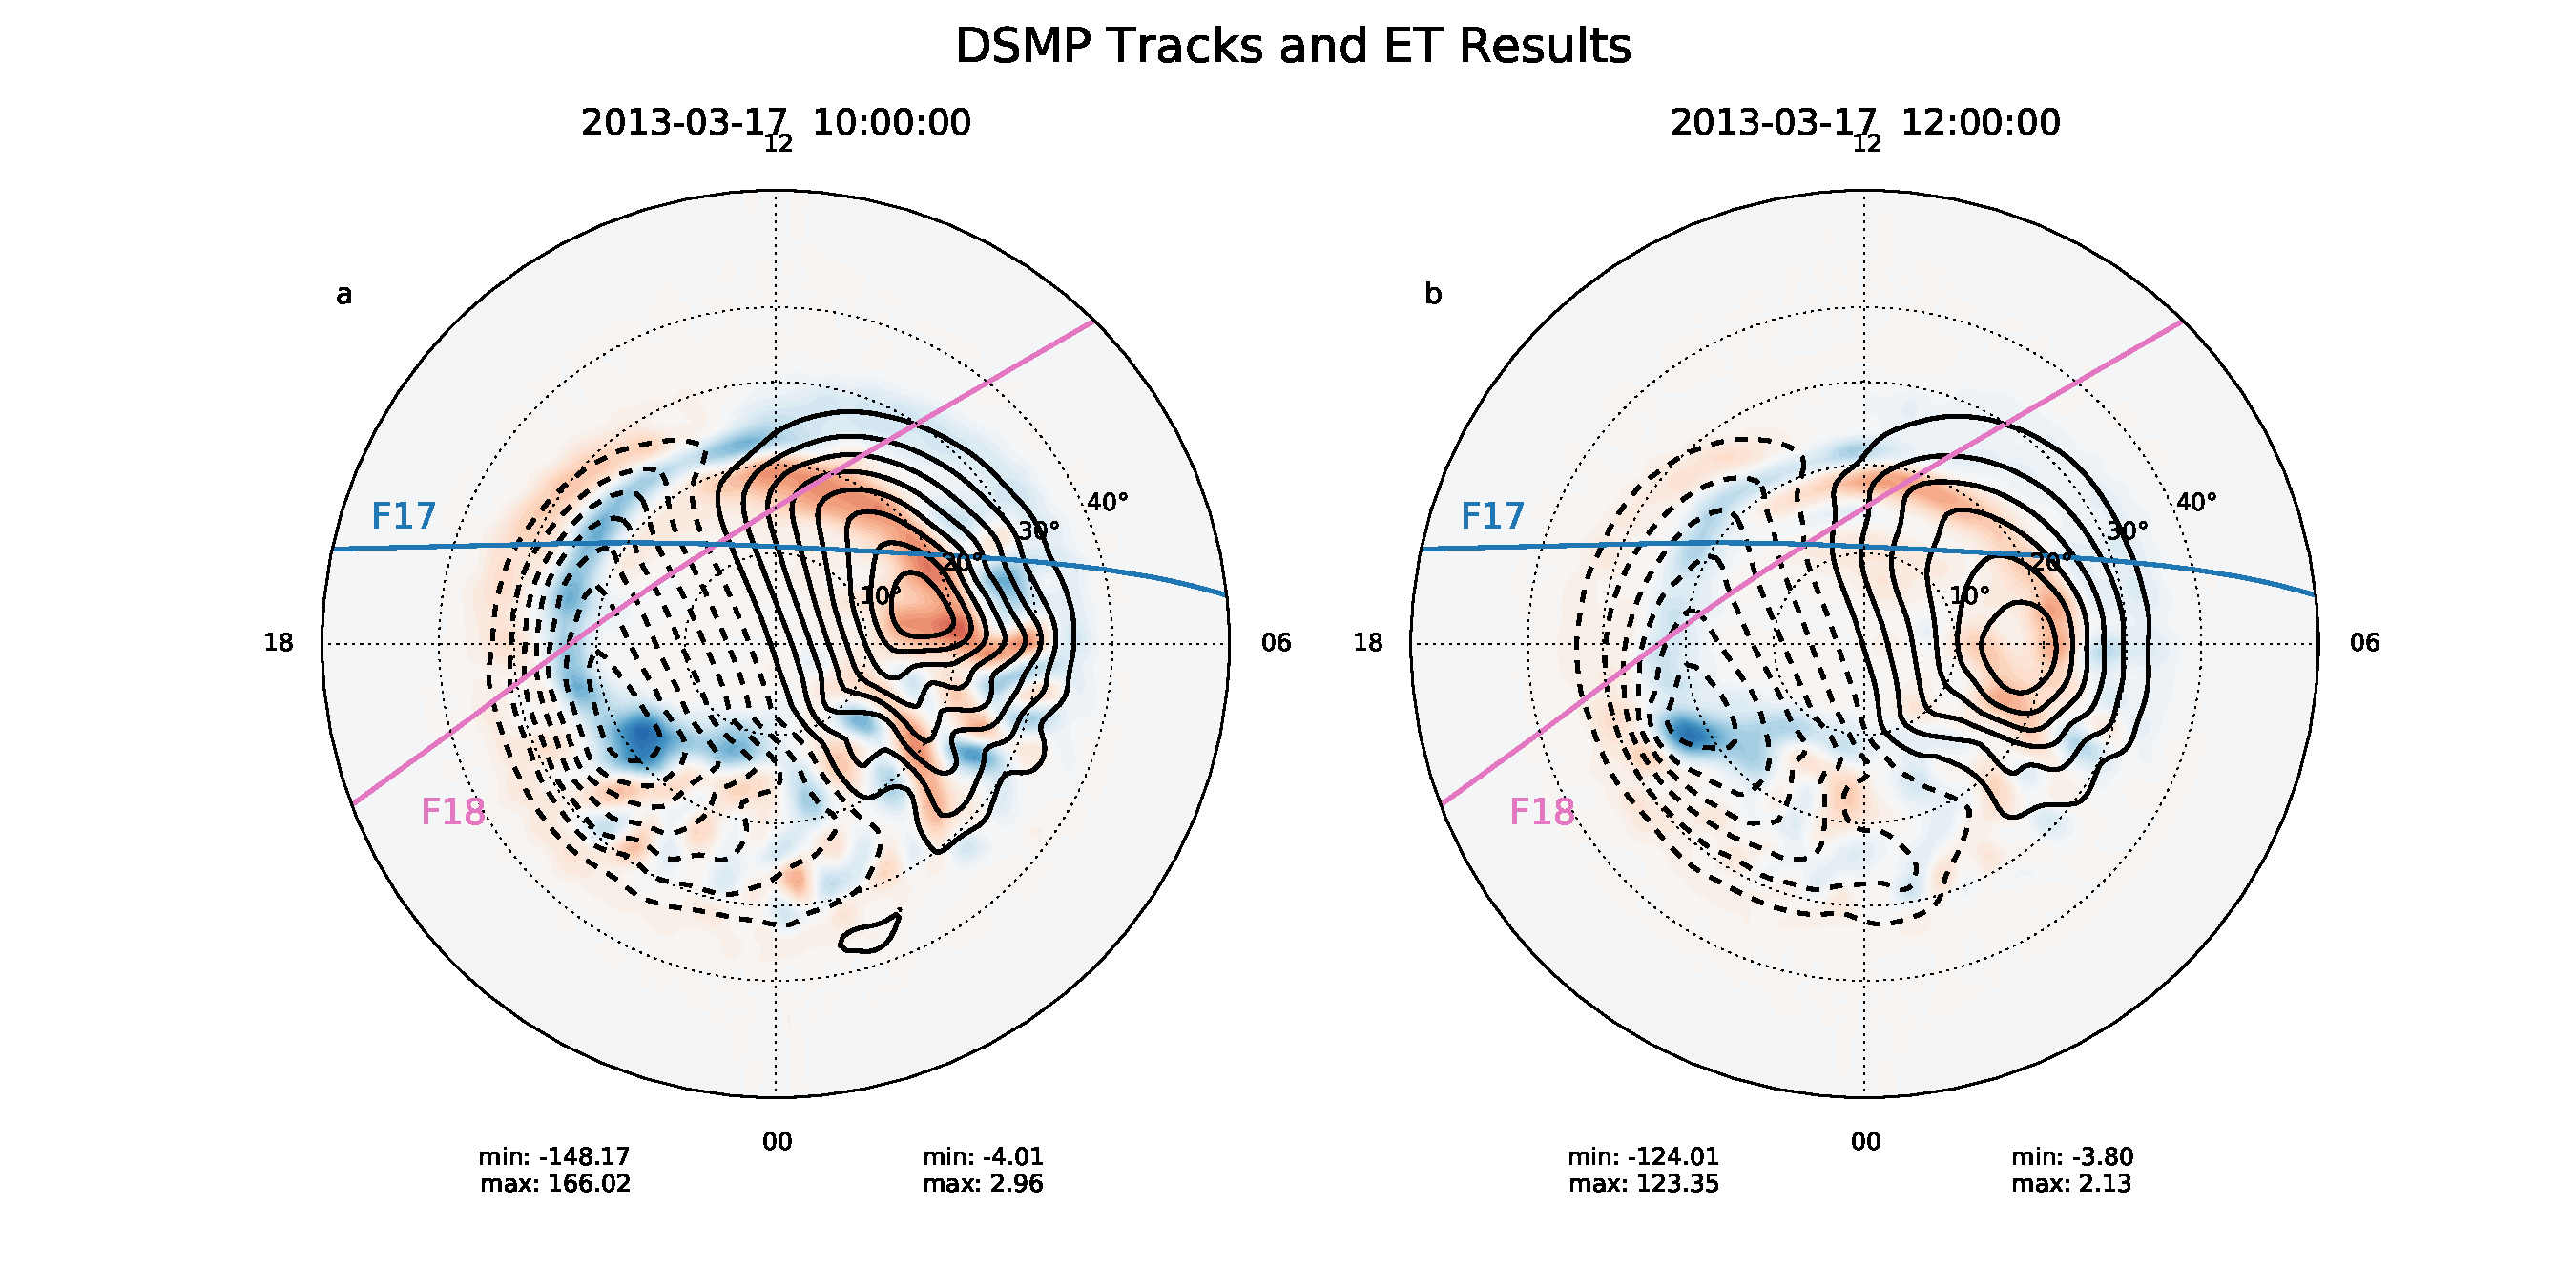
\includegraphics[width=39pc]{JGR-DMSPTraj.pdf}
\caption{\label{dmsptraj-fig}
DSMP F17 and F18 trajectories overlaid on top of ET FAC and CPCP patterns.  Panel a shows the F17 trajectory between 0945 and 1030 UT and the F18 trajectory between 1000 and 1045 UT overlaid on top of the ET simulation results for 10:00UT.   Panel b shows the F17 trajectory between 1125 and 1210 UT and the F18 trajectory between 1145 and 1230 UT overlaid on top of the ET simulation results for 12:00UT.  In each panel the F17 trajectory is blue and the F18 trajectory is pink.}
\end{figure*}

The panels a and c of Figure \ref{f17-comp-fig} show comparisons on the cross-track ion drift velocity between the DMSP measurements and the simulations along two consecutive orbits of the F17 spacecraft over the northern hemisphere, orbiting from the duskside to dawnside across the polar region. The velocity shown in Figure \ref{f17-comp-fig} is perpendicular to the satellite trajectory, with positive values for anti-sunward convection and negative values for sunward convection. As indicated by the measured drift velocity in Figure \ref{f17-comp-fig}, the DMSP F17 satellite passes through the regions of two-cell convection with sunward drift in the dusk sector, followed by anti-sunward drift over the polar cap and sunward drift in the dawn sector. The b and d of Figure \ref{f17-comp-fig} show the measured spectrum of electron and ion precipitation. The measured equatorward boundaries of the auroral oval are indicated using black dashed lines in each panel based on the sharp gradient in the observed electron spectrum. According to the DMSP drift velocity and particle measurements, the observed double-channel profiles of the westward drift velocity on the dusk side (near 9:59 and 11:41 UT) are separated by the auroral precipitation boundary in both cases, indicating that the lower latitude westward plasma flow is in the subauroral region, which is also known as sub-auroral polarization streams (SAPS). The comparisons on the cross-track plasma drift velocity suggest that the coupled LFM-RCM model is capable of reproducing the large-scale two-cell convection velocity profiles observed along the two consecutive DMSP F17 trajectories. As indicated by the boundaries of the simulated auroral energy flux  the spatial extension of the simulated auroral oval resembles the observations during the two F17 passes. Combined with the simulated velocity profiles, the LFM-RCM model is also capable of reproducing the magnitude of the observed fast plasma flow in the subauroral region (during 09:54-10:00 and 11:34-11:40) with little particle precipitation fluxes.
 
\begin{figure*}[t]
\noindent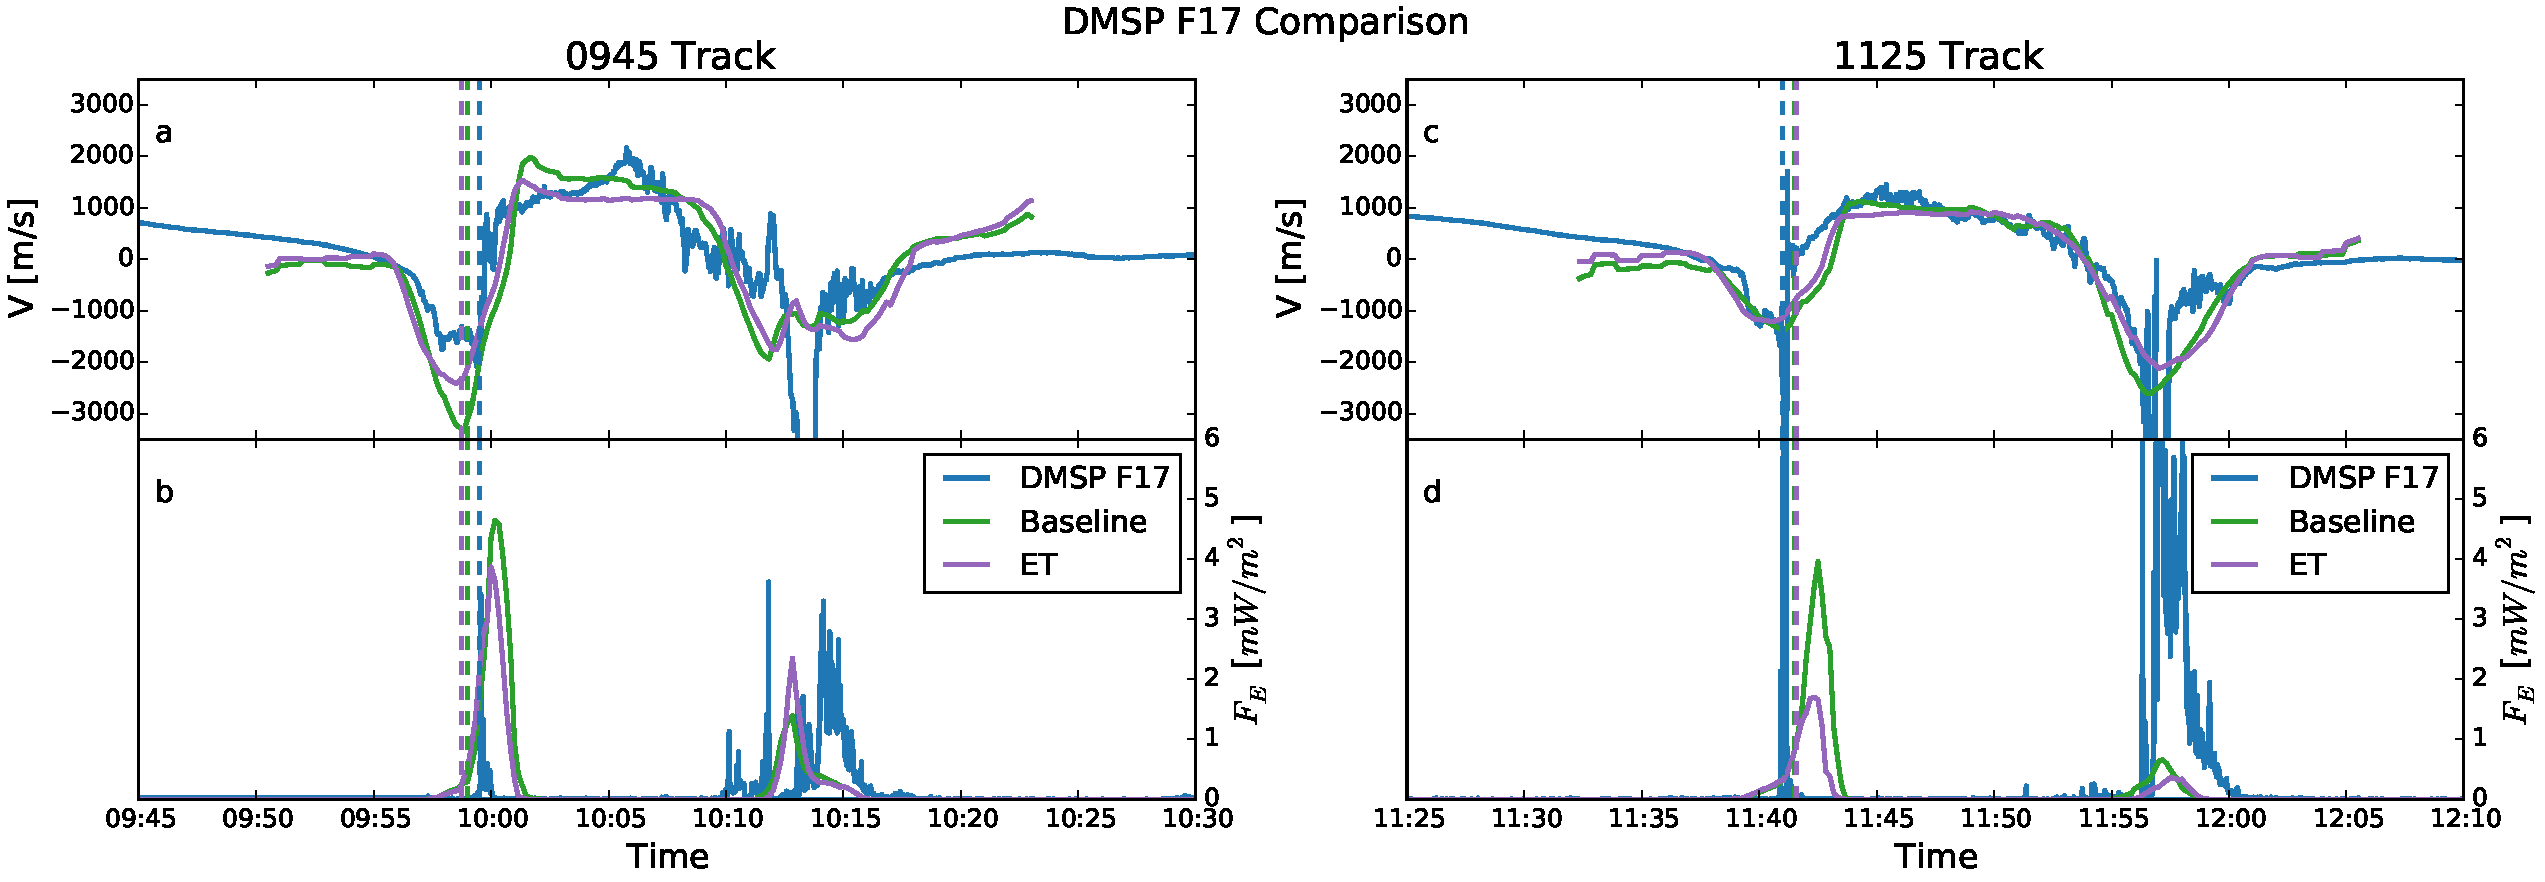
\includegraphics[width=39pc]{JGR-DMSPF17.pdf}
\caption{\label{f17-comp-fig}
Comparison of DMSP F17 observations and simulation results.  The first column, panels a and b, show the comparison for the 0945 pass.  The second column, panels c and d, have the comparison for the 1125 pass.  The first row, panels a and c, compare the cross track ion velocity from DMSP with the velocities obtained from the Baseline and ET simulations.  The second row, panels b and d, compares the electron energy fluxes.  In each panel the observations are show in blue, the baseline results in green and ET results in purple.}
\end{figure*}

A similar comparison between the LFM-RCM simulation and the measurements from two consecutive DMSP F18 passes during the main phase of the storm is shown in Figure \ref{f18-comp-fig}. The LFM-RCM model is capable of reproducing the double-channel convection profiles during both F18 trajectories between 10:09-10-18 and 11:54-12:03 UT, respectively, although the simulated peak location of the subauroral flow channel is a couple of degrees MLAT poleward compared to the measured SAPS features especially during the second F18 pass. It is possible that the location discrepancies in the SAPS channel between the LFM-RCM simulation and DMSP observations are due to the fact that the auroral oval in the LFM-RCM simulation is several degrees of MLAT poleward compared to the measured particle spectrum. The disagreement in the location of the auroral oval is likely a consequence of the fact that the distribution of upward Region 1 field-aligned currents in the global simulation is several degrees in MLAT poleward compared to observations (reference Zhang et al., 2011, or comparison with Weimer in this paper?). Note that on the dawnside, the LFM-RCM simulation misses the channels of anti-sunward flow observed by the two DMSP F18 passes near 10:27 and 12:12 UT, which is possibly due to the fact that the simulated high-latitude convection pattern in LFM-RCM is more contract than the measurements in the morning sector (reference to the statistical study?). 

\begin{figure*}[t]
\noindent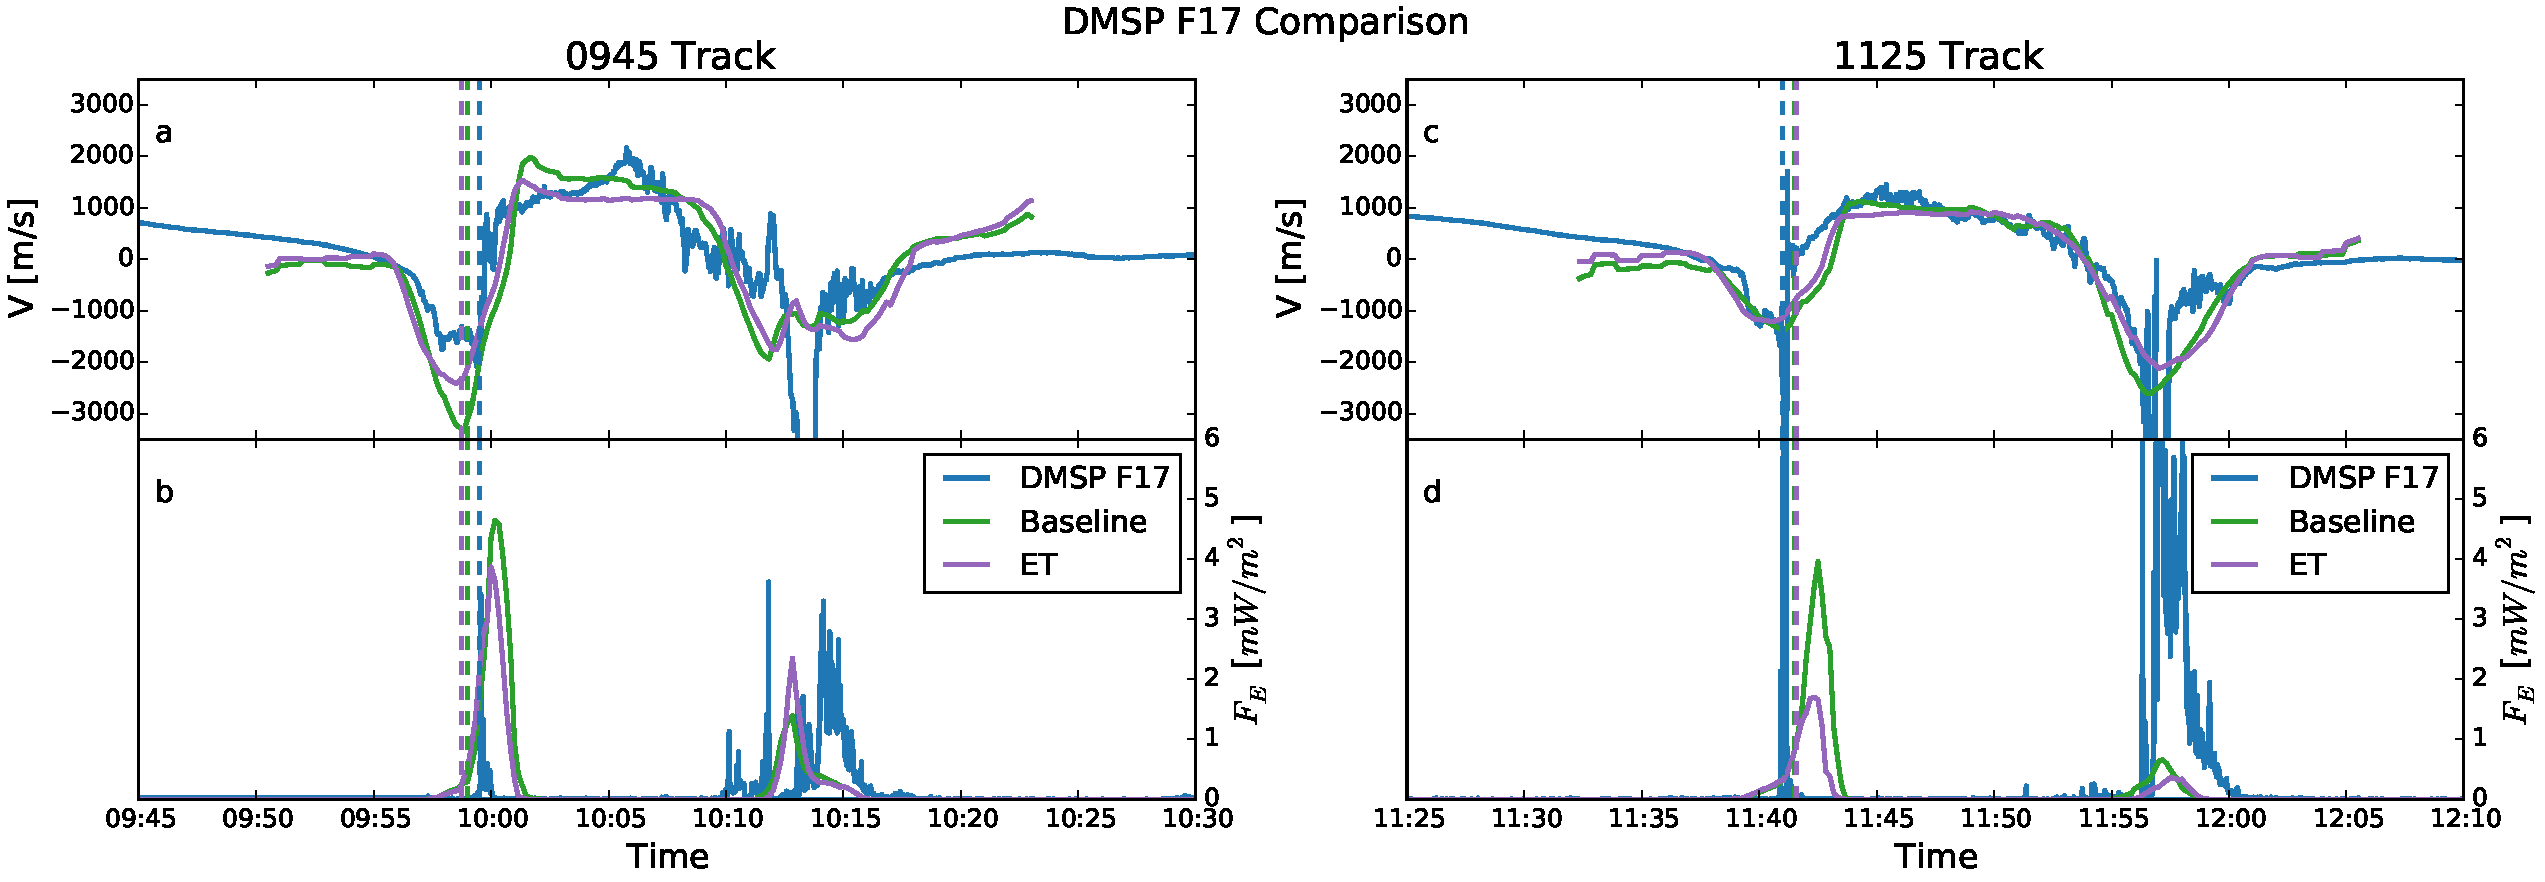
\includegraphics[width=39pc]{JGR-DMSPF17.pdf}
\caption{\label{f18-comp-fig}
Comparison for DSMP F18 observations in the same format as Figure \ref{f17-comp-fig}.}
\end{figure*}

 \subsection{Comparison with AMPERE}
 \label{sec-ampere}

Now we move onto a comparison of the simulation results with the observations of the FAC patterns obtained from the AMPERE mission.  The second scientific visualization accompanying this paper makes this comparison by plotting the patterns of the northern hemisphere currents along with cuts along specific MLTs. Figure \ref{ampere-comp-fig} is extracted from this visualization at 09:00 UT on March 17th.  The top row in the visualization provides a comparison of the FAC patterns for the northern hemisphere from the simulation and the AMPERE reconstruction.  A two minute cadence was adopted for this visualization to match the highest output frequency available for the AMPERE observations.  It is important to note that the AMPERE observations are built up over a 10 minute averaging window and that average is being compared with an instantaneous value obtain from the MIX output.  {\em Slava - Please confirm that my description of the AMPERE reconstruction method is correct.}  In order to allow for a more quantitative comparison the bottom row of the visualization contains cuts from the current densities at several magnetic local times.  Panels d and f provide cuts through the morning and afternoon sectors while panel e provides a cut from dusk to dawn.  

\begin{figure*}[t]
\noindent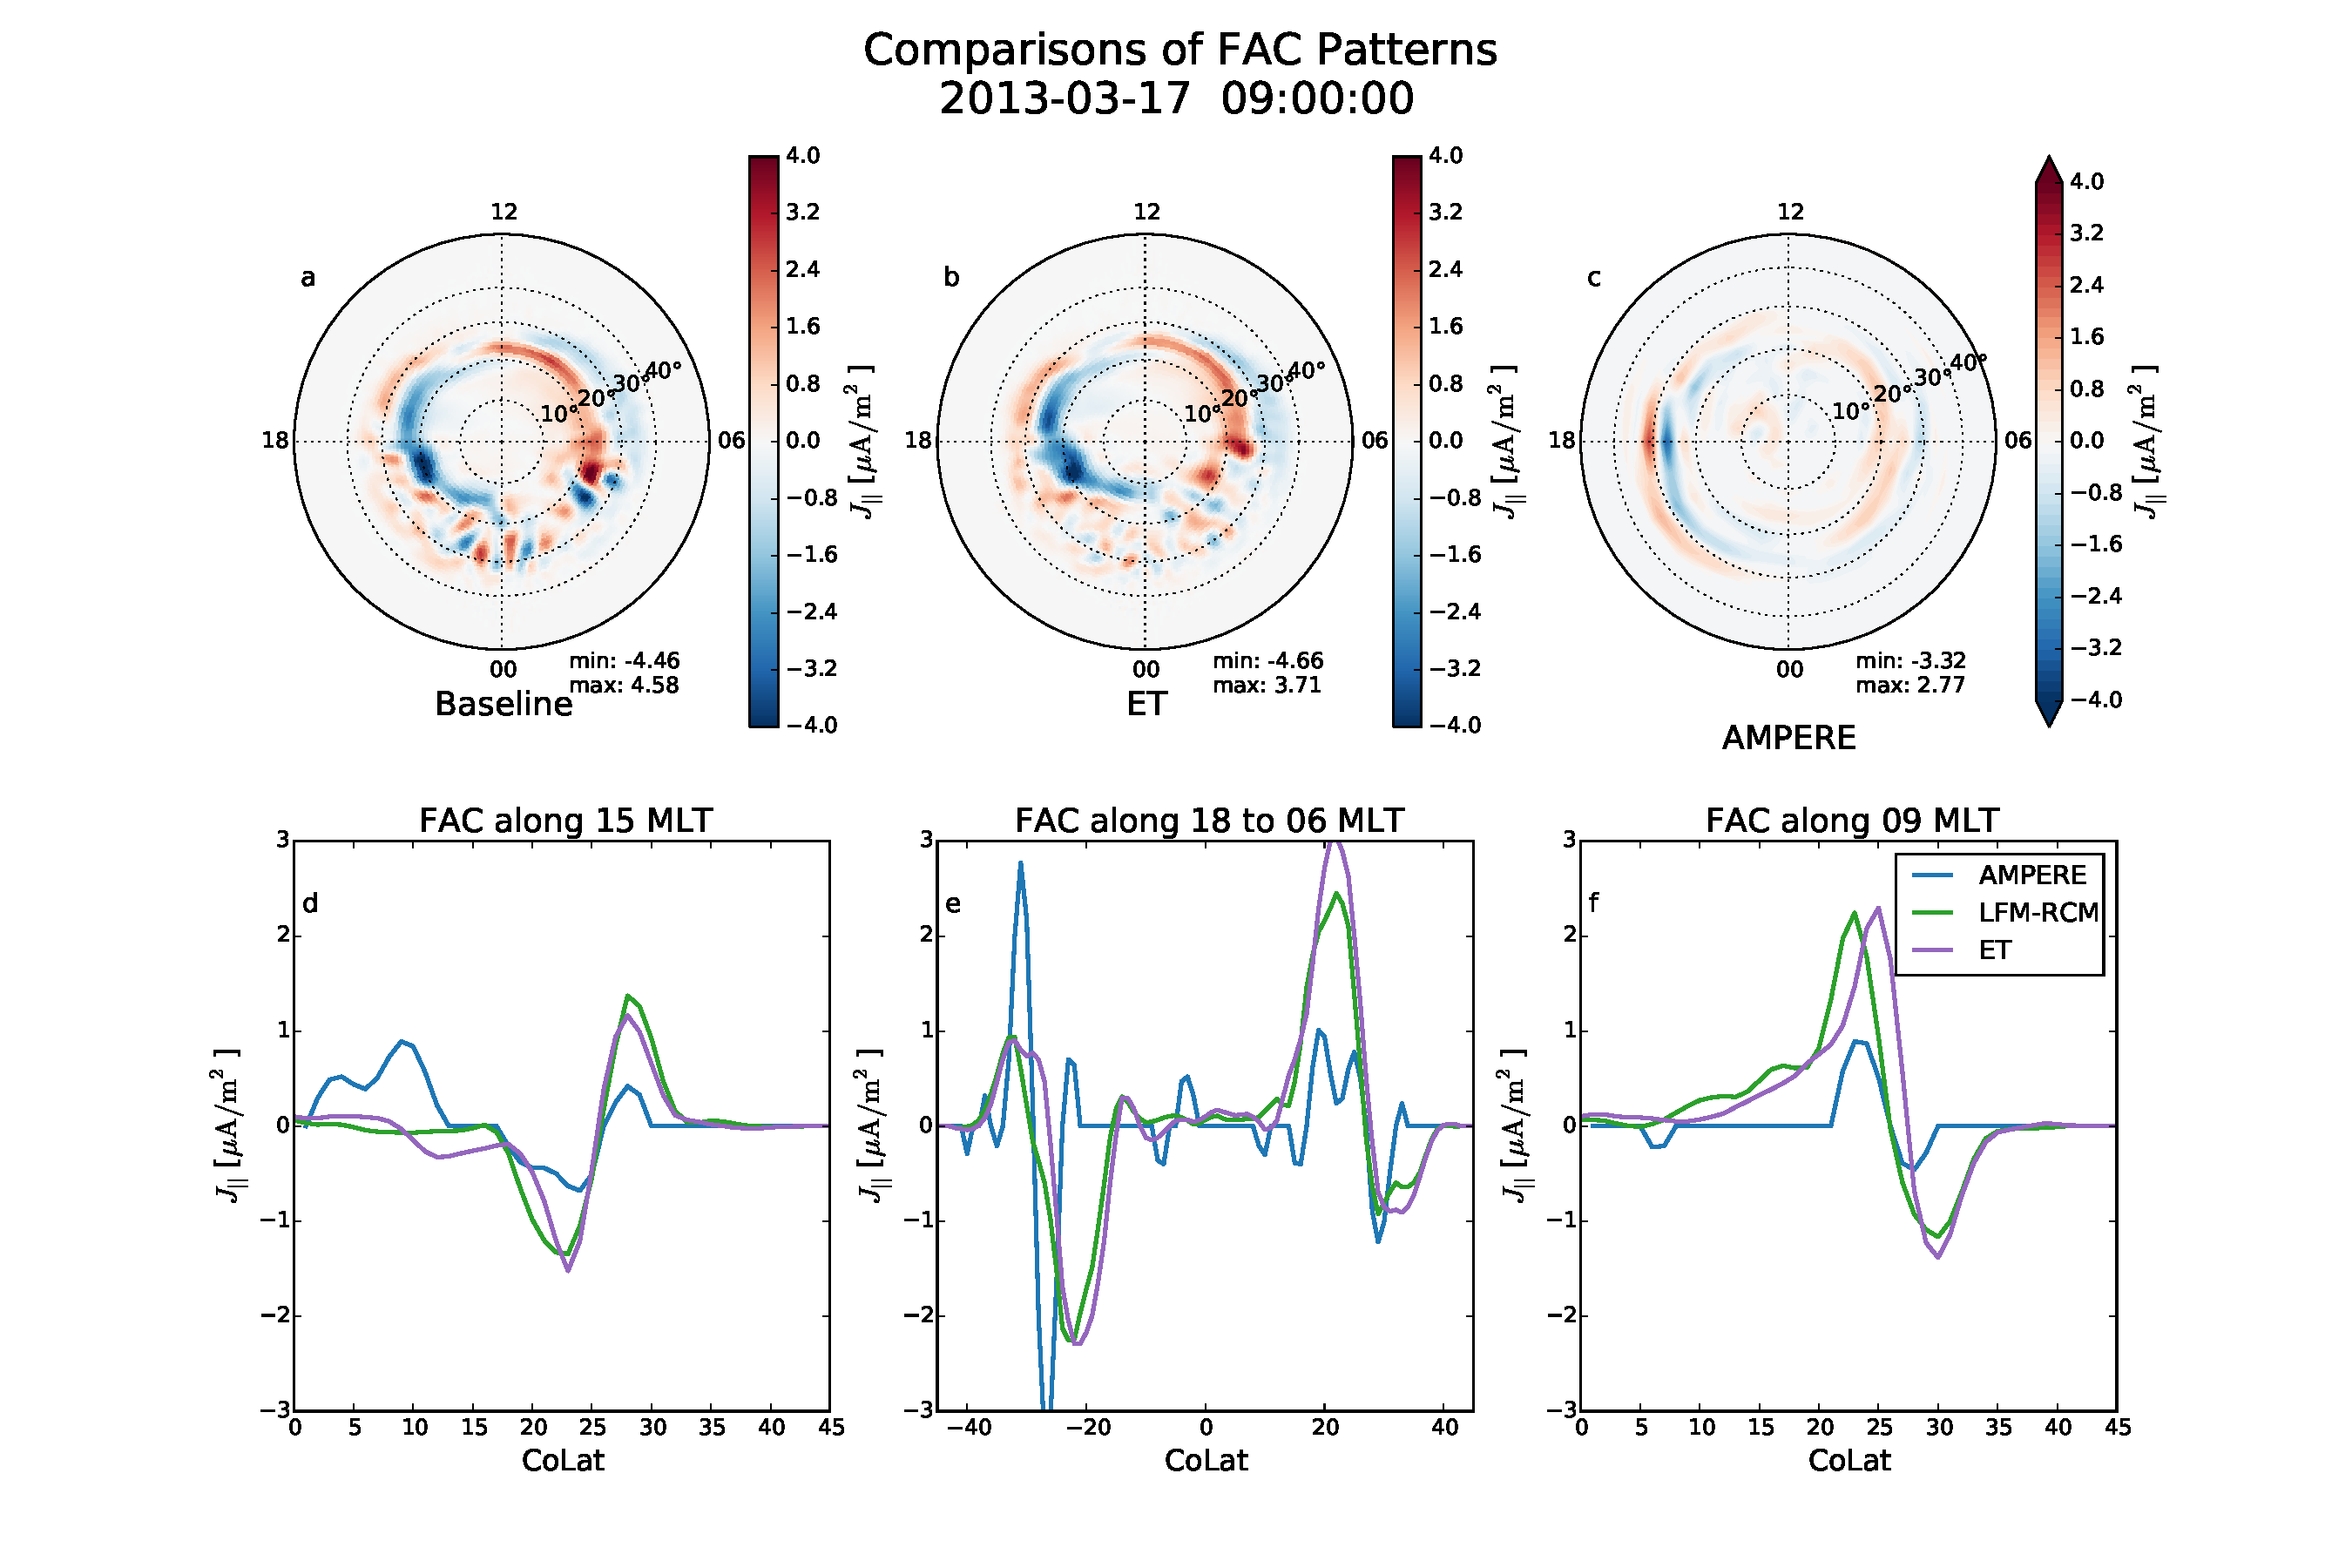
\includegraphics[width=39pc]{JGR-AmpereComparison.pdf}
\caption{\label{ampere-comp-fig}
Frame extracted from the scientific visualization comparing the FAC from the simulations with the patterns derived from AMPERE magnetometer observations.  The top row, panels a-c, shows the FAC patterns for the northern hemisphere using the same color bar.  Panel a is the baseline simulation, panel b is the from the Electrojet Turbulence simulation and panel c is from the AMPERE observations.  The bottom row makes comparisons of current strengths along cuts in MLT.  Panel d is a cut along 15 MLT and extends from 0-45 degrees colatitude.   Panel f is cut along 09 MLT and has the same range as panel a.  Panel is a cut along the 18 and 06 MLT line.  In this plot the negative colatitude values correspond to locations along the 18 MLT line, while the positive values are along the 06 MLT line.  This plot gives a cut from dusk to dawn in a single panel.  In all the comparison plots the AMPERE observations are shown in blue, the baseline simulation in green and the ET simulation in purple.}
\end{figure*}

As discussed in Section \ref{sec-comp} prior to the arrival of the shock the solar wind driving of the magnetosphere is quite weak.  At 03:00 UT the solar IMF is mainly northward and a careful examination of the FAC patterns at this time shows an NBZ current system in both simulation results.  The faint trace of an NBZ current system is apparent in the afternoon sector.  These patterns can be hard to see in the visualization since the range of the color bar was selected to capture times when strong currents are flowing.  Turning our attention to the MLT comparisons we see that for the 09 and 15 MLT cuts the two simulation results are virtually identical.  Differences can be seen in the 18 MLT portion of the dawn-dusk cut, due the current in the ET version extending slightly more anti-sunward.  The NBZ current systems do not appear in the AMPERE reconstruction, especially since a threshold value of 0.15 [$\mu A m^{-2}$] is needed for the currents to above the noise threshold.  The strong level agreement between the two simulations is not surprising since the ET effects are not likely to occur at this point in the simulation.

Next we focus our attention at 09:00 UT shown in Figure \ref{ampere-comp-fig} that corresponds to time with the largest differences in CPCP seen between the two simulation results and is occurring at time of strong driving of the magnetosphere.  While the difference between the CPCP is largest at this time there is a striking level of similarity in the FAC patterns for the two simulations.  Across the entire days side the location, width, and strengths of the R1 and R2 currents are quite similar.  There is a notable difference on the nightside with the baseline simulation have stronger FAC pairs in the midnight sector.  Also the peaks in the R1 currents that occur below the 18-06 MLT line are stronger in the baseline simulation.  The strength of the currents is stronger than those seen in the AMPERE results.  The R1 and R2 currents also appear to be at higher latitudes than those seen in the AMPERE results.  The weaker currents in the AMPERE results has been reported before by \cite{2013JGRA..118.4977M} and is result of the fitting process underestimating the true current strength.  Looking at the 15 MLT comparison we see that the strength of currents along this cut is the same in the baseline and ET simulations.  The current peaks are higher and about a 1-2 degrees higher in latitude.  There is also a high latitude feature in the AMPERE current observations that does not appear in either simulation result.  In the 09 MLT there is a 1-2 degree difference in the location of the peak current between the two simulation results.  The current peaks appear to bracket the observed current peak with the baseline simulation peak at above the AMPERE peak and the ET peak below it.   The peak current here is about a factor of two larger than the AMPERE results and the currents are wider.  The wider currents in the simulation results are also seen in the 18-06 MLT cut.  This especially clear for the currents in the 18 MLT line.  Unlike the other currents reported here the AMPERE currents are stronger in this region than what is reported by AMPERE.  Along the 06 MLT cut the currents return to being about a factor of 2 larger in the R1 location.  Even though is this the time with largest difference in CPCP the differences between the two simulations is relatively modest and agree quite well with the AMPERE observations.

As previously noted as the storm progress through the remainder of the day there are intervals with strong driving a differences between the CPCP between the two simulations.  The 14:00 UT frame is typical of the conditions during the 13:30-14:35 interval of strong driving.  The modest 1-2 degree separation between the current peaks noted in the 09 MLT cut of the 09:00 UT is present in all of the cuts through the currents.  In general, the baseline simulation peak appears to be closer to the peak in the AMPERE observations.  This trend is also apparent in the 15:45-19:30 UT interval of strong driving with the 16:12 frame providing a clear example.  Also notable in this frame are the strong peaks in the R1 currents below the 18-06 MLT line in the ET simulation results.  It is worth pointing out that at 13:26 UT time, previously identified as an instant with little differences between the CPCP and integrated FAC there are very small differences between the two simulation results. 


 \subsection{Comparison with TS07-D}
 \label{sec-ts07d}
 Initial drafting of this section has been assigned to Slava.
 
 
 May include a comparison with pressures in the in the ring current depending on length and quality of comparison.
 
\begin{figure*}[t]
\noindent\includegraphics[width=39pc]{PressureComparison.png}
\caption{\label{press-fig}
Temporary Figure comparing Baseline and ET pressures}
\end{figure*}


 \section{Summary and Future Directions}
\label{sec-future}

Mike will write this section once the paper is nearly finished.

Our SAPS are the best!


%%% End of body of article:

%%%%%%%%%%%%%%%%%%%%%%%%%%%%%%%%
%% Optional Appendix goes here
%
% \appendix resets counters and redefines section heads
% but doesn't print anything.
% After typing  \appendix
%
% \section{Here Is Appendix Title}
% will show
% Appendix A: Here Is Appendix Title
%
%%%%%%%%%%%%%%%%%%%%%%%%%%%%%%%%%%%%%%%%%%%%%%%%%%%%%%%%%%%%%%%%
%
% Optional Glossary or Notation section, goes here
%
%%%%%%%%%%%%%%
% Glossary is only allowed in Reviews of Geophysics
% \section*{Glossary}
% \paragraph{Term}
% Term Definition here
%
%%%%%%%%%%%%%%
% Notation -- End each entry with a period.
% \begin{notation}
% Term & definition.\\
% Second term & second definition.\\
% \end{notation}
%%%%%%%%%%%%%%%%%%%%%%%%%%%%%%%%%%%%%%%%%%%%%%%%%%%%%%%%%%%%%%%%
%
%  ACKNOWLEDGMENTS

\begin{acknowledgments}
This material is based upon work supported by NASA grants XX, YY, and ZZ.  The National Center for Atmospheric Research is sponsored by the National Science Foundation.  All model output, simulation codes, and analysis routines are being preserved on the NCAR High Performance Storage System and will be made available upon written request to the lead author of this publication. 
\end{acknowledgments}

%% ------------------------------------------------------------------------ %%
%%  REFERENCE LIST AND TEXT CITATIONS
%
% Either type in your references using
% \begin{thebibliography}{}
% \bibitem{}
% Text
% \end{thebibliography}
%
% Or,
%
% If you use BiBTeX for your references, please use the agufull08.bst file (available at % ftp://ftp.agu.org/journals/latex/journals/Manuscript-Preparation/) to produce your .bbl
% file and copy the contents into your paper here.
%
% Follow these steps:
% 1. Run LaTeX on your LaTeX file.
%
% 2. Make sure the bibliography style appears as \bibliographystyle{agu08full}. Run BiBTeX on your LaTeX 
% file.
%
% 3. Open the new .bbl file containing the reference list and
%   copy all the contents into your LaTeX file here.
%
% 4. Comment out the old \bibliographystyle and \bibliography commands.
%
% 5. Run LaTeX on your new file before submitting.
%
% AGU does not want a .bib or a .bbl file. Please copy in the contents of your .bbl file here.

%\begin{thebibliography}{}

%\providecommand{\natexlab}[1]{#1}
%\expandafter\ifx\csname urlstyle\endcsname\relax
%  \providecommand{\doi}[1]{doi:\discretionary{}{}{}#1}\else
%  \providecommand{\doi}{doi:\discretionary{}{}{}\begingroup
%  \urlstyle{rm}\Url}\fi
%
%\bibitem[{\textit{Atkinson and Sloan}(1991)}]{AtkinsonSloan}
%Atkinson, K., and I.~Sloan (1991), The numerical solution of first-kind
%  logarithmic-kernel integral equations on smooth open arcs, \textit{Math.
%  Comp.}, \textit{56}(193), 119--139.
%
%\bibitem[{\textit{Colton and Kress}(1983)}]{ColtonKress1}
%Colton, D., and R.~Kress (1983), \textit{Integral Equation Methods in
%  Scattering Theory}, John Wiley, New York.
%
%\bibitem[{\textit{Hsiao et~al.}(1991)\textit{Hsiao, Stephan, and
%  Wendland}}]{StephanHsiao}
%Hsiao, G.~C., E.~P. Stephan, and W.~L. Wendland (1991), On the {D}irichlet
%  problem in elasticity for a domain exterior to an arc, \textit{J. Comput.
%  Appl. Math.}, \textit{34}(1), 1--19.
%
%\bibitem[{\textit{Lu and Ando}(2012)}]{LuAndo}
%Lu, P., and M.~Ando (2012), Difference of scattering geometrical optics
%  components and line integrals of currents in modified edge representation,
%  \textit{Radio Sci.}, \textit{47},  RS3007, \doi{10.1029/2011RS004899}.
%\end{thebibliography}

\bibliographystyle{agu08}
\bibliography{papers-full}
%Reference citation examples:

%...as shown by \textit{Kilby} [2008].
%...as shown by {\textit  {Lewin}} [1976], {\textit  {Carson}} [1986], {\textit  {Bartholdy and Billi}} [2002], and {\textit  {Rinaldi}} [2003].
%...has been shown [\textit{Kilby et al.}, 2008].
%...has been shown [{\textit  {Lewin}}, 1976; {\textit  {Carson}}, 1986; {\textit  {Bartholdy and Billi}}, 2002; {\textit  {Rinaldi}}, 2003].
%...has been shown [e.g., {\textit  {Lewin}}, 1976; {\textit  {Carson}}, 1986; {\textit  {Bartholdy and Billi}}, 2002; {\textit  {Rinaldi}}, 2003].

%...as shown by \citet{jskilby}.
%...as shown by \citet{lewin76}, \citet{carson86}, \citet{bartoldy02}, and \citet{rinaldi03}.
%...has been shown \citet{jskilbye}.
%...has been shown \citet{lewin76,carson86,bartoldy02,rinaldi03}.
%...has been shown \citet [e.g.,][]{lewin76,carson86,bartoldy02,rinaldi03}.
%
% Please use ONLY \citet and \citet for reference citations.
% DO NOT use other cite commands (e.g., \cite, \citeyear, \nocite, \citealp, etc.).

%% ------------------------------------------------------------------------ %%
%
%  END ARTICLE
%
%% ------------------------------------------------------------------------ %%
\newpage
\end{article}

%% Enter Figures and Tables here:

% When submitting articles through the GEMS system:
% COMMENT OUT ANY COMMANDS THAT INCLUDE GRAPHICS.
%
% DO NOT USE \psfrag or \subfigure commands.
%
% Figure captions go below the figure.
% Table titles go above tables; all other caption information
%  should be placed in footnotes below the table.

% DRAFT figure/table, including eps graphics
%
% \begin{figure}
% \noindent\includegraphics[width=20pc]{samplefigure.eps}
% \caption{Caption text here}
% \end{figure}
% \end{document}
%
% \begin{table}
% \caption{}
% \end{table}
%
% ---------------
% TWO-COLUMN figure/table
%
% \begin{figure*}
% \noindent\includegraphics[width=39pc]{samplefigure.eps}
% \caption{Caption text here}
% \end{figure*}
%
% \begin{table*}
% \caption{Caption text here}
% \end{table*}
%
% ---------------
% EXAMPLE TABLE
%
%\begin{table}
%\caption{Time of the Transition Between Phase 1 and Phase 2\tablenotemark{a}}
%\centering
%\begin{tabular}{l c}
%\hline
% Run  & Time (min)  \\
%\hline
%  $l1$  & 260   \\
%  $l2$  & 300   \\
%  $l3$  & 340   \\
%  $h1$  & 270   \\
%  $h2$  & 250   \\
%  $h3$  & 380   \\
%  $r1$  & 370   \\
%  $r2$  & 390   \\
%\hline
%\end{tabular}
%\tablenotetext{a}{Footnote text here.}
%\end{table}










% See below for how to make landscape/sideways figures or tables.

\end{document}

%%%%%%%%%%%%%%%%%%%%%%%%%%%%%%%%%%%%%%%%%%%%%%%%%%%%%%%%%%%%%%%

More Information and Advice:

%% ------------------------------------------------------------------------ %%
%
%  SECTION HEADS
%
%% ------------------------------------------------------------------------ %%

% Capitalize the first letter of each word (except for
% prepositions, conjunctions, and articles that are
% three or fewer letters).

% AGU follows standard outline style; therefore, there cannot be a section 1 without
% a section 2, or a section 2.3.1 without a section 2.3.2.
% Please make sure your section numbers are balanced.
% ---------------
% Level 1 head
%
% Use the \section{} command to identify level 1 heads;
% type the appropriate head wording between the curly
% brackets, as shown below.
%
%An example:
%\section{Level 1 Head: Introduction}
%
% ---------------
% Level 2 head
%
% Use the \subsection{} command to identify level 2 heads.
%An example:
%\subsection{Level 2 Head}
%
% ---------------
% Level 3 head
%
% Use the \subsubsection{} command to identify level 3 heads
%An example:
%\subsubsection{Level 3 Head}
%
%---------------
% Level 4 head
%
% Use the \subsubsubsection{} command to identify level 3 heads
% An example:
%\subsubsubsection{Level 4 Head} An example.
%
%% ------------------------------------------------------------------------ %%
%
%  IN-TEXT LISTS
%
%% ------------------------------------------------------------------------ %%
%
% Do not use bulleted lists; enumerated lists are okay.
% \begin{enumerate}
% \item
% \item
% \item
% \end{enumerate}
%
%% ------------------------------------------------------------------------ %%
%
%  EQUATIONS
%
%% ------------------------------------------------------------------------ %%

% Single-line equations are centered.
% Equation arrays will appear left-aligned.

Math coded inside display math mode \[ ...\]
 will not be numbered, e.g.,:
 \[ x^2=y^2 + z^2\]

 Math coded inside \begin{equation} and \end{equation} will
 be automatically numbered, e.g.,:
 \begin{equation}
 x^2=y^2 + z^2
 \end{equation}

% IF YOU HAVE MULTI-LINE EQUATIONS, PLEASE
% BREAK THE EQUATIONS INTO TWO OR MORE LINES
% OF SINGLE COLUMN WIDTH (20 pc, 8.3 cm)
% using double backslashes (\\).

% To create multiline equations, use the
% \begin{eqnarray} and \end{eqnarray} environment
% as demonstrated below.
\begin{eqnarray}
  x_{1} & = & (x - x_{0}) \cos \Theta \nonumber \\
        && + (y - y_{0}) \sin \Theta  \nonumber \\
  y_{1} & = & -(x - x_{0}) \sin \Theta \nonumber \\
        && + (y - y_{0}) \cos \Theta.
\end{eqnarray}

%If you don't want an equation number, use the star form:
%\begin{eqnarray*}...\end{eqnarray*}

% Break each line at a sign of operation
% (+, -, etc.) if possible, with the sign of operation
% on the new line.

% Indent second and subsequent lines to align with
% the first character following the equal sign on the
% first line.

% Use an \hspace{} command to insert horizontal space
% into your equation if necessary. Place an appropriate
% unit of measure between the curly braces, e.g.
% \hspace{1in}; you may have to experiment to achieve
% the correct amount of space.


%% ------------------------------------------------------------------------ %%
%
%  EQUATION NUMBERING: COUNTER
%
%% ------------------------------------------------------------------------ %%

% You may change equation numbering by resetting
% the equation counter or by explicitly numbering
% an equation.

% To explicitly number an equation, type \eqnum{}
% (with the desired number between the brackets)
% after the \begin{equation} or \begin{eqnarray}
% command.  The \eqnum{} command will affect only
% the equation it appears with; LaTeX will number
% any equations appearing later in the manuscript
% according to the equation counter.
%

% If you have a multiline equation that needs only
% one equation number, use a \nonumber command in
% front of the double backslashes (\\) as shown in
% the multiline equation above.

%% ------------------------------------------------------------------------ %%
%
%  LANDSCAPE/SIDEWAYS FIGURE AND TABLE EXAMPLES
%
%% ------------------------------------------------------------------------ %%
%
% For figures, add \usepackage{lscape} to the file and the landscape.sty style file
% to the paper folder.
%
% \begin{figure*}[p]
% \begin{landscapefigure*}
% Illustration here.
% \caption{caption here}
% \end{landscapefigure*}
% \end{figure*}
%
% For tables, add \usepackage{rotating} to the paper and add the rotating.sty file to the folder.
%
% AGU prefers the use of {sidewaystable} over {landscapetable} as it causes fewer problems.
%
% \begin{sidewaystable}
% \caption{}
% \begin{tabular}
% Table layout here.
% \end{tabular}
% \end{sidewaystable}
%
%

